\documentclass[english]{article}
\usepackage{notestemplate}
\usepackage{for}

\begin{document}

\makecover{Foundations of Operations Research}{2022/2023}

% TODO find a title for all the properties OR use a environment for each
% https://www.overleaf.com/learn/latex/Theorems_and_proofs#Reference_guide

\section{Introduction}

\subsection{Algorithm}

An algorithm for a problem is a sequence of instructions that allows to solve any of its instances.
The execution time of an algorithm depends on various factors, most notably the instance and the computer.

\bigskip
\textbf{Properties}:

\begin{itemize}
  \item An algorithm is \textbf{exact} if it provides an optimal solution for every instance.
        \begin{itemize}
          \item otherwise is \textbf{heuristic}
        \end{itemize}
  \item A \textbf{greedy algorithm} constructs a feasible solution iteratively, by making at each step a \textit{locally optimal} choice, without reconsidering previous choices
        \begin{itemize}
          \item for most \textit{discrete optimization problems}, greedy type algorithms yield a feasible solution with no guarantee of optimality
        \end{itemize}
\end{itemize}

\subsection{Dynamic Programming}

Proposed by \textit{Richard Bellman} in \(1950\), \textbf{dynamic programming} \textit{(or \DP)} is a method for solving optimization problems, composed of a sequence of decisions, by solving a set of recursive equations.

\DP is applicable to any sequential decision problem, for which the optimality property is satisfied;
as such, it has a wide range of applications, including scheduling, transportation, and assignment problems.

\subsection{Complexity of algorithms}

In order analyze an algorithm, it's necessary to consider its complexity as a function of the size of the instance \textit{(the size of the input)}, independently of the computer;
the complexity is defined as the number of elementary operations by assuming that each elementary operation takes a constant time.

Since it's hard to determine the exact number of elementary operations, an additional assumption is made: only the asymptotic number of elementary operations in the worst case (for the worst instances) is considered.
The complexity evaluation is then performed by looking for the function \(f(n)\) that best approximates the upper bound on the number of elementary operations \(n\) for the worst instances.

\subsubsection{Big-O notation}

A function \(f\) if order of \(g\), written \(f(n) = \bigO{g(n)}\) if exists a constant \(c > 0\) and a constant \(n_0 > 0\) such that \(f(n) \leq c \cdot g(n)\) for all \(n \geq n_0\).

An illustration of the big-O notation is shown in Figure~\ref{fig:big-o-notation}.

\begin{figure}[htbp]
  \bigskip
  \centering
  \tikzfig{figure-1.tikz}
  \caption{Big-O notation}
  \label{fig:big-o-notation}
  \bigskip
\end{figure}

\subsection{Complexity classes}

Two classes of algorithms are considered, according to their worst case order of complexity:

\begin{itemize}
  \item \textbf{Polynomial}: \(\bigO{n^d}\) for a constant \(d > 0, d \in \R\)
  \item \textbf{Exponential}: \(\bigO{d^n}\) for a constant \(d > 0, d \in \R\)
\end{itemize}

Algorithms with a hight order Polynomial complexity are not considered efficient.

A comparison of the two classes, assuming that \(1 \, \mu s\) is needed for each elementary operation, is shown in Table~\ref{tab:complexity-classes}.

\begin{table}
  \centering
  \bigskip
  \begin{tblr}{c|c|c}
    \(n\)  & \(n^2\)          & \(2^n\)                \\
    \hline
    \(1\)  & \(1 \, \mu s\)   & \(1 \, \mu s\)         \\
    \(10\) & \(100 \, \mu s\) & \(1.024 \, ms\)        \\
    \(20\) & \(400 \, \mu s\) & \(\approx 1.04\, s\)   \\
    \(30\) & \(900 \, \mu s\) & \(\approx 18 \, m\)    \\
    \(40\) & \(1.6 \, ms\)    & \(\approx 13 \, d\)    \\
    \(50\) & \(2.5 \, ms\)    & \(\approx 36 \, y\)    \\
    \(60\) & \(3.6 \, ms\)    & \(\approx 36535 \, y\) \\
  \end{tblr}
  \caption{Complexity classes}
  \label{tab:complexity-classes}
  \bigskip
\end{table}

\clearpage

\section{Graph and Network Optimization}

Many \textbf{decision making problems} can be formulated in terms of graphs and networks, such as:

\begin{itemize}
  \item \textbf{transportation} and \textbf{distribution} problems
  \item \textbf{network design} problems
  \item \textbf{location} problem
  \item timetable \textbf{scheduling}
  \item \ldots
\end{itemize}

\subsection{Graphs}

A \textbf{graph} is a pair \(G = (N, E)\) with:

\begin{itemize}
  \item \(N\) a set of \textbf{nodes} or \textbf{vertices}
  \item \(E \subseteq N \times N\) a set of \textbf{edges} or arcs connecting them pairwise
        \begin{itemize}
          \item A \textbf{directed} graph is a graph in which set set \(E\) is composed by ordered pairs of distinct nodes
                \begin{itemize}[label=\(\rightarrow\)]
                  \item an edge connecting nodes \(i\) and \(j\) is represented by \(\{i, j\}\)
                  \item the flow is permitted only in the direction of the arrow \textit{(from \(i\) to \(j\))}
                  \item \(i\) is the head of the arc and \(j\) is the tail
                \end{itemize}
          \item A \textbf{undirected} graph is a graph in which set set \(E\) is composed by unordered pairs of distinct nodes
                \begin{itemize}[label=\(\rightarrow\)]
                  \item an edge connecting nodes \(i\) and \(j\) is represented by \((i, j)\)
                  \item since all edges are undirected, \((i, j)\) is equivalent to \((j, i)\)
                \end{itemize}
        \end{itemize}
\end{itemize}

\bigskip
\textbf{Properties}:

\begin{itemize}
  \item Two \textbf{nodes} \(i\) and \(j\) are \textbf{adjacent} if they are connected by an edge \((i, j)\) or \(\{i, j\}\)
  \item An \textbf{edge} \(e\) is \textbf{incident} in a node \(v\) if \(v\) is an \textbf{endpoint} of \(e\)
        \begin{itemize}
          \item \textbf{undirected} graphs: the degree of a node is the number of incident edges
          \item \textbf{directed} graphs: the in-degree \textit{(out-degree)} of a node is the number of arcs that have it as successor \textit{(predecessor)}
        \end{itemize}
  \item A \textbf{path} from \(i \in N \text{ to } j \in N\) is a sequence of edges in a undirected graph
        \[ p = \left\langle \{v_1, v_2\}, \{v_2, v_3\}, \ldots, \{v_{k-1}, v_k\}\right\rangle \]
        connecting nodes \(v_1, \ldots, v_k\), with \(\{v_i, v_{i+1} \in E\}\) for \(i = 1, \ldots, k-1\)
  \item A \textbf{directed path} \(i \in N \text{ to } j \in N\) is a sequence of arcs in a directed graph
        \[ p = \left\langle (v_1, v_2), (v_2, v_3), \ldots, (v_{k-1}, v_k)\right\rangle \]
        connecting nodes, with  \((v_i, v_{i+1} \in E)\)  for \(i = 1, \ldots, k-1\)
  \item A \textbf{cycle} is a path \[ \left\langle v_1, v_2, \ldots, v_1 \right\rangle \] where the first and last nodes are the same
        \begin{itemize}
          \item A \textbf{directed cycle} is path \[ \left\langle \{v_1, v_2\}, \{v_2, v_3\}, \ldots, \{v_{k-1}, v_k\}, \{v_k, v_1\}\right\rangle \]
                where the first and the last nodes are the same
        \end{itemize}
  \item Nodes \(u\) and \(v\) are \textbf{connected} if exists a path connecting them
  \item A graph \((N, E)\) is \textbf{connected} if \(u, v\) are connecting \(\forall \, u, v \in N\)
        \begin{itemize}
          \item A graph \((N, E)\) is \textbf{strongly connected} if \(u, v\) are connected by a \textbf{directed} path \(\forall \, u, v \in N\)
        \end{itemize}
  \item A graph is \textbf{bipartite} if there is a partition \(N = N_1 \cup N_2, \, N_1 \cap N_2 = \emptyset\) such that \(\forall \, (u, v) \in E, u \in N_1 \text{ and } v \in N_2\)
  \item A graph is \textbf{complete} if \(E = \left\{\{v_i, v_j\} \,|\, v_i, v_j \in N \land i \leq j \right\}\)
  \item Given a directed graph \(G = (N, A)\) and \(S \subseteq N\), the \textbf{outgoing cut} induced by \(S\) is the set of arcs:
        \[\delta^+(S) = \left\{ (u, v) \in A \,|\, u \in S \land v \in N \setminus S \right\}\]
        the \textbf{incoming cut} induced by \(S\) is the set of arcs:
        \[\delta^-(S) = \left\{ (u, v) \in A \,|\, v \in S \land u \in N \setminus S \right\}\]
  \item A graph with \(n\) \textbf{nodes} has at most \(m = \dfrac{n(n-1)}{2}\) \textbf{edges}
  \item A \textbf{directed} graph with \(n\) \textbf{nodes} has at most \(m = n(n-1)\) \textbf{arcs}
        \begin{itemize}
          \item a graph is \textbf{dense} if \(m \approx n^2\)
          \item a graph is \textbf{sparse} if \(m \ll n\)
        \end{itemize}
  \item The adjacency list \(A(i)\) of a node \(i\) is the set of arcs emanating from that node
        \[ A(i) = \left\{ j \in N \mid   (i, j) \in A  \right\} \]
\end{itemize}

\bigskip
Some examples are shown in Figure \ref{fig:examples-of-graphs}.

\begin{figure}[htbp]
  \centering
  \begin{subfigure}[t]{0.495\textwidth}
    \centering
    \begin{tikzpicture}[node distance = 2cm, minimum size = 0.75cm]
      \samplegraph
      \sampleedges
    \end{tikzpicture}
    \caption{Undirected graph}
    \label{fig:undirected-graph}
  \end{subfigure}
  \begin{subfigure}[t]{0.495\textwidth}
    \centering
    \begin{tikzpicture}[node distance = 2cm, minimum size = 0.75cm]
      \samplegraph
      \samplearcs
    \end{tikzpicture}
    \caption{Directed graph}
    \label{subfig:directed-graph}
  \end{subfigure}
  \bigskip
  \begin{subfigure}[t]{0.495\textwidth}
    \centering
    \begin{tikzpicture}[node distance = 2cm, minimum size = 0.75cm]
      \samplegraph

      \path[-] (1) edge (2);
      \path[-] (1) edge (4);
      \path[-][color=red] (2) edge (3);
      \path[-] (2) edge (4);
      \path[-][color=red] (3) edge (4);
      \path[-] (3) edge (5);
      \path[-][color=red] (4) edge (5);
    \end{tikzpicture}
    \caption{\shortstack{Connected graph, nodes \(2\) and \(5\) are connected \\ \(\langle \{2, 3\}, \{3, 4\}, \{4, 5\} \rangle\) is a path}}
    \label{subfig:connected-graph}
  \end{subfigure}
  \begin{subfigure}[t]{0.495\textwidth}
    \centering
    \begin{tikzpicture}[circle, node distance = 2cm, minimum size = 0.75cm]
      \samplegraph

      \path[->] (1) edge (2);
      \path[->] (1) edge (4);
      \path[->, color=red] (2) edge (3);
      \path[->, color=red] (3) edge (4);
      \path[->, color=red] (3) edge (5);
      \path[->, color=red] (4) edge (2);
      \path[->] (4) edge[bend left=15] (5);
      \path[->, color=red] (5) edge[bend left=15] (4);
    \end{tikzpicture}
    \caption{\shortstack{Not strongly connected graph \\ \(\langle \{3, 5\}, \{5, 4\}, \{4, 2\}, \{2, 3\}, \{3, 4\} \rangle\) is a directed path}}
    \label{subfig:not-strongly-connected-graph}
  \end{subfigure}
  \bigskip
  \begin{subfigure}[t]{0.495\textwidth}
    \centering
    \begin{tikzpicture}[circle, node distance = 2cm, minimum size = 0.75cm]
      \samplegraph

      \path[-] (1) edge (2);
      \path[-] (1) edge (4);
      \path[-, color=red] (2) edge (3);
      \path[-, color=red] (2) edge (4);
      \path[-] (3) edge (4);
      \path[-, color=red] (3) edge (5);
      \path[-, color=red] (4) edge (5);
    \end{tikzpicture}
    \caption{\shortstack{Cycle \\ \(\langle \{2, 3\}, \{3, 5\}, \{5, 4\}, \{4, 2\}\rangle\) is a cycle}}
    \label{subfig:cycle}
  \end{subfigure}
  \begin{subfigure}[t]{0.495\textwidth}
    \centering
    \begin{tikzpicture}[circle, node distance = 2cm, minimum size = 0.75cm]
      \samplegraph

      \path[->] (1) edge (2);
      \path[->] (1) edge (4);
      \path[->, color=red] (2) edge (3);
      \path[->, color=red] (3) edge (4);
      \path[->] (3) edge (5);
      \path[->, color=red] (4) edge (2);
      \path[->] (4) edge[bend left=15] (5);
      \path[->] (5) edge[bend left=15] (4);
    \end{tikzpicture}
    \caption{\shortstack{Circuit \\ \(\langle (2, 3), (3, 4), (4, 2)\)} is a circuit}
    \label{subfig:circuit}
  \end{subfigure}
  \bigskip
  \begin{subfigure}[t]{0.495\textwidth}
    \centering
    \begin{tikzpicture}[circle, node distance = 2cm, minimum size = 0.75cm]
      \samplegraph

      \path[-] (3) edge (5);
      \path[-] (5) edge (1);
      \path[-] (1) edge (4);
      \path[-] (4) edge (2);
    \end{tikzpicture}
    \caption{\shortstack{Bipartite graph \\ \(N_1 = \left\{1, 2, 3\right\}, N_2 = \left\{4, 5\right\}\)}}
    \label{subfig:bipartite-graph}
  \end{subfigure}
  \begin{subfigure}[t]{0.495\textwidth}
    \centering
    \begin{tikzpicture}[circle, node distance = 2cm, minimum size = 0.75cm]
      \samplegraph

      \path[-] (2) edge (3);
      \path[-] (3) edge (4);
      \path[-] (4) edge (2);
      \path[-] (1) edge (2);
      \path[-] (1) edge (3);
      \path[-] (1) edge (4);
    \end{tikzpicture}
    \caption{\shortstack{Complete graph \\ \(N = \left\{1, 2, 3, 4\right\}\)}}
    \label{subfig:complete-graph}
  \end{subfigure}
  \bigskip
  \begin{subfigure}[t]{0.99\textwidth}
    \centering
    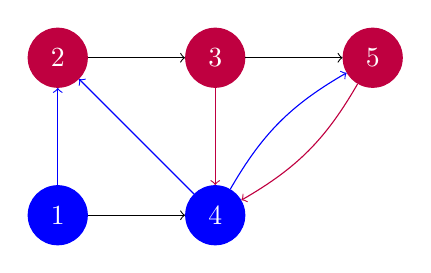
\begin{tikzpicture}[circle, node distance = 2cm, minimum size = 0.75cm]
      \node[draw, fill=purple, draw=purple, text=white] (2) {2};
      \node[draw, fill=purple, draw=purple, text=white] (3) [right of = 2] {3};
      \node[draw, fill=purple, draw=purple, text=white] (5) [right of = 3] {5};
      \node[draw, fill=blue, draw=blue, text=white] (1) [below of = 2] {1};
      \node[draw, fill=blue, draw=blue, text=white] (4) [below of = 3] {4};

      \path[->, color=blue] (1) edge (2);
      \path[->, color=blue] (4) edge (2);
      \path[->, color=blue] (4) edge [bend left=15] (5);

      \path[->, color=purple] (3) edge (4);
      \path[->, color=purple] (5) edge [bend left=15] (4);

      \path[->] (2) edge (3);
      \path[->] (3) edge (5);
      \path[->] (1) edge (4);
    \end{tikzpicture}
    \caption{incoming (\(\delta^+\)) and outgoing (\(\delta^-\)) cuts of two sets of nodes \textit{(purple and blue)}}
    \label{subfig:incoming-outgoing-cuts}
  \end{subfigure}
  \caption{Examples of graphs}
  \label{fig:examples-of-graphs}
\end{figure}

\subsubsection{Graphs representation}

Graphs are represented by:

\begin{itemize}
  \item Adjacency \textbf{matrix} \(\mathbf{A}\) of size \(n \times n\) if the graph is \textbf{dense}
        \[ a_{ij} = \begin{cases} 1 \ &\text{if } (i, j) \in A\\ a_{i_j} &\text{otherwise}\end{cases} \]
  \item Adjacency \textbf{list} \(\mathbf{A}\) of size \(n\) if the graph is \textbf{sparse}
\end{itemize}

The same representation can be used for both directed and undirected graphs;
the adjacency matrix for an undirected graph is \textbf{symmetric}.

\bigskip
An example of a graph representation is shown in Figure~\ref{fig:graph-representation}.

\begin{figure}[htbp]
  \begin{subfigure}{0.33\textwidth}
    \centering
    \begin{tikzpicture}[circle, node distance = 2cm, minimum size = 0.75cm]
      \samplegraph

      \path[->] (1) edge (2);
      \path[->] (1) edge (4);
      \path[->] (2) edge (3);
      \path[->] (3) edge (4);
      \path[->] (3) edge (5);
      \path[->] (4) edge (2);
      \path[->] (4) edge[bend left=15] (5);
      \path[->] (5) edge[bend left=15] (4);
    \end{tikzpicture}
    \caption{Graph}
  \end{subfigure}
  \begin{subfigure}{0.33\textwidth}
    \centering
    \(A = \begin{bmatrix}
      0 & 1 & 0 & 1 & 0 \\
      0 & 0 & 1 & 0 & 0 \\
      0 & 0 & 0 & 1 & 1 \\
      0 & 1 & 0 & 0 & 1 \\
      0 & 0 & 0 & 1 & 0
    \end{bmatrix}\)
    \caption{Adjacency matrix}
  \end{subfigure}
  \begin{subfigure}{0.33\textwidth}
    \centering
    \(\begin{matrix}
      S(1) = \left\{2, 4\right\} \\
      S(2) = \left\{3\right\}    \\
      S(3) = \left\{4, 5\right\} \\
      S(4) = \left\{2, 5\right\} \\
      S(5) = \left\{4\right\}
    \end{matrix}\)
    \caption{Adjacency list}
  \end{subfigure}
  \caption{Graph representation}
  \label{fig:graph-representation}
\end{figure}

\subsubsection{Graph reachability problem}

\begin{problem}[graph reachability]
Given a directed graph \(G = (N, A)\) and a node \(s \in N\), the \textbf{graph reachability problem} consists in finding all nodes reachable from \(s\).
\end{problem}

\bigskip
\textbf{Goal}
\begin{itemize}[label=\(\rightarrow\)]
  \item \textit{Input}: graph \(G = (N, A)\), described via successor lists, and a node \(s \in N\)
  \item \textit{Output}: subset \(M \subseteq N\) of nodes of \(G\) reachable from \(s\)
\end{itemize}

The goal is reached by an \textit{efficient} algorithm to solve the problem, with the following properties:
\begin{itemize}
  \item a \textbf{queue} \(Q\) of nodes not yet processed is kept by the algorithm
  \item the queue uses a \texttt{FIFO} policy
  \item the nodes exploration is performed in a \textbf{breadth-first} manner
\end{itemize}

\bigskip
\textbf{Algorithm}
The algorithm pseudocode is shown in Code~\ref{lst:graph-reachability}.

\begin{lstlisting}[caption={Graph reachability}, label={lst:graph-reachability}, float]
Q := {s}
M := {}
while Q is not empty do
  u := node $\in$ Q
  Q := Q \ {u}
  M := M $\cup$ {u}
  for (u, v) $\in \ \delta^+(\texttt{u})$ do
    if v $\notin$ M and v $\notin$ Q then
      Q := Q $\cup$ {v}
    end
  end
end
\end{lstlisting}

The algorithm stops when \(\delta^+(M) = \emptyset\) \textit{(when the outgoing cut of the set of nodes \(M\) is empty)};
\(\delta^-(M)\) is the set of arcs with head node in \(M\) and tail in \(N \setminus M\).

\paragraph{Complexity analysis}

At each iteration of the \texttt{\textbf{while}} loop:

\begin{enumerate}
  \item A node \(u\) is \textbf{removed} from the queue \(Q\) and \textbf{added} to the set \(M\)
  \item For all nodes \(v\) directly reachable from \(u\) and not already in \(M\) or \(Q\), \(v\) is added to \(Q\)
\end{enumerate}

Since each node \(u\) is inserted in \(Q\) at most once and each arch \((u,v)\) is considered at most once, the overall complexity is:
\[ \bigO{n+m} \quad n = |N|, \ m =|A|\]
For dense graphs, this value converges to \(\bigO{n^2}\).

\subsection{Subgraphs and Trees}

Let \(G = (N, E)\) be a graph.
Then:

\begin{itemize}
  \item \(G^\prime = (N^\prime, E^\prime)\) is a \textbf{subgraph} of \(G\) if \(N^\prime \subseteq N\) and \(E^\prime \subseteq E\)
  \item A \textbf{tree} \(G_T = (N^\prime, T)\) of \(G\) is a connected, acyclic, subgraph of \(G\)
  \item \(G_T = (N^\prime, T)\) is a \textbf{spanning tree} of \(G\) if it contains all the nodes \textit{(\(N^\prime = N\))}
  \item The \textbf{leaves} of a tree are the nodes with degree \(1\)
\end{itemize}

\bigskip
A representation of these concepts is shown in Figure~\ref{fig:subgraphs-trees}.

\begin{figure}[htbp]
  \centering
  \begin{subfigure}[t]{0.995\textwidth}
    \centering
    \begin{tikzpicture}[node distance = 2cm, minimum size = 0.75cm]
      \samplegraph
      \sampleedges
    \end{tikzpicture}
    \caption{Graph \(G\)}
  \end{subfigure}
  \bigskip
  \begin{subfigure}[t]{0.3\textwidth}
    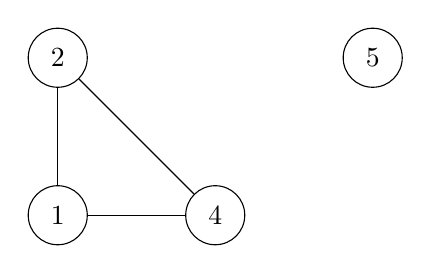
\begin{tikzpicture}[circle, node distance = 2cm, minimum size = 0.75cm]
      \node[draw] (2) {2};
      \node[] (3) [right of = 2] {};
      \node[draw] (5) [right of = 3] {5};
      \node[draw] (1) [below of = 2] {1};
      \node[draw] (4) [below of = 3] {4};

      \path[-] (2) edge (4);
      \path[-] (4) edge (1);
      \path[-] (1) edge (2);
    \end{tikzpicture}
    \caption{Subgraph \(G^\prime\) of \(G\)}
  \end{subfigure}
  \begin{subfigure}[t]{0.3\textwidth}
    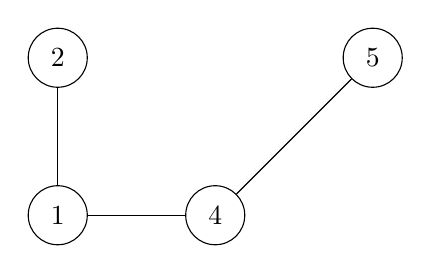
\begin{tikzpicture}[circle, node distance = 2cm, minimum size = 0.75cm]
      \node[draw] (2) {2};
      \node[] (3) [right of = 2] {};
      \node[draw] (5) [right of = 3] {5};
      \node[draw] (1) [below of = 2] {1};
      \node[draw] (4) [below of = 3] {4};

      \path[-] (5) edge (4);
      \path[-] (4) edge (1);
      \path[-] (1) edge (2);
    \end{tikzpicture}
    \caption{Subgraph \(G^{\prime\prime}\) of \(G\) and a tree}
  \end{subfigure}
  \begin{subfigure}[t]{0.3\textwidth}
    \begin{tikzpicture}[circle, node distance = 2cm, minimum size = 0.75cm]
      \samplegraph

      \path[-] (1) edge (4);
      \path[-] (2) edge (4);
      \path[-] (2) edge (3);
      \path[-] (4) edge (5);
    \end{tikzpicture}
    \caption{Subgraph \(G^{\prime\prime}\) of \(G\) and a tree}
  \end{subfigure}
  \caption{Subgraphs and trees}
  \label{fig:subgraphs-trees}
\end{figure}

\subsection{Properties of trees}

\begin{property}[Number of edges]
  Every tree with \(n\) nodes has \(n-1\) edges.
\end{property}

\begin{proof}
  \hfill
  \begin{itemize}
    \item \textbf{Base case}: the claim holds for \(n=1\) \textit{(a tree with a single node has no edges)}
    \item \textbf{Inductive steps}: show that the claim is valid for for any tree with \(n + 1\) nodes
          \begin{itemize}
            \item let \(T_1\) be a tree with \(n+1\) and recall with any tree with \(n \geq 2\) nodes has at least \(2\) leaves
            \item by deleting one of the leaves and its incident edge, a tree \(T_2\) with \(n\) nodes is obtained
            \item by induction hypothesis, \(T_2\) has \(n-1\) edges; therefore, \(T_1\) has \(n-1+1=n\) edges
          \end{itemize}
  \end{itemize}
\end{proof}

\begin{property}
  Any pair of nodes in a tree is connected via a unique path.
  Otherwise, the tree would contain a cycle.
  \label{prop:number-of-paths}
\end{property}

\begin{property}
  By adding a new edge to a tree, a new unique cycle is created.
  This cycle consists of the path created in Property~\ref{prop:number-of-paths} and the new edge.
\end{property}

\begin{property}
  Let \(G_T = (N, T)\) be a spanning tree of \(G = (N, E)\).
  Consider an edge \(e \notin T\) and the unique cycle \(C\) of \(T \cup \{e\}\).
  For each edge \(f \in C \setminus \{e\}\), the subgraph \(T \cup \{e\} \setminus \{f\}\) is a spanning tree of \(G\).
\end{property}

\begin{figure}[htbp]
  \centering
  \bigskip
  \begin{subfigure}[t]{0.495\textwidth}
    \centering
    \begin{tikzpicture}[circle, node distance = 2cm, minimum size = 0.75cm]
      \samplegraph
      \path[-] (1) edge (2);
      \path[-] (2) edge (3);
      \path[-, text=red, color=red] (3) edge node[above]{\(f\)} (5);
      \path[-] (5) edge (4);
      \path[-, text=blue,color=blue] (4) edge node[above]{\(e\)} (2);
    \end{tikzpicture}
    \caption{Graph \(G_T\), edge \(f\) is red, edge \(e\) is blue}
  \end{subfigure}
  \begin{subfigure}[t]{0.495\textwidth}
    \centering
    \begin{tikzpicture}[circle, node distance = 2cm, minimum size = 0.75cm]
      \samplegraph

      \path[-] (1) edge (2);
      \path[-] (2) edge (3);
      \path[-] (3) edge (5);
      \path[-] (5) edge (4);
    \end{tikzpicture}
    \caption{\(T \cup \{e\} \setminus \{f\}\)}
  \end{subfigure}
  \caption{Exchange property}
  \label{fig:exchange-property}
  \bigskip
\end{figure}

\begin{property}
  Let \(F\) be a partial tree \textit{(spanning nodes in \(S \subseteq N\))} contained in a optimal spanning tree of \(G = (N, E)\).
  Consider \(e = \left\{u, v\right\} \in \delta(S)\) of minimum cost, then there exists a minimum cost spanning tree of \(G\) containing \(e\).
\end{property}

\begin{proof}
  By contradiction, assume \(T^\ast \subseteq E\) is a minimum cost spanning tree with \(F \subseteq T^\ast\) and \(e \notin T^\ast\).

  Adding an edge \(e\) to \(T^\ast\) creates the cycle \(C\).
  Let \(f \in \delta(S) \cap C\):

  \begin{itemize}
    \item If \(c_e = c_f\), then \(T^\ast \cup \{e\}\setminus \{f\}\) is a minimum cost spanning tree of \(G\) as it has the same cost as \(T^\ast\)
    \item If \(c_e < c_f\), then \(c \left( T^\ast \cup \{e\} \setminus \{f\} \right) < c \left(T^\ast\right)\), hence \(T^\ast\) is not optimal
  \end{itemize}

\end{proof}

\newpage

\subsection{Optimal cost spanning tree}

\textbf{Spanning trees} have a number of applications, including:

\begin{itemize}
  \item \textbf{network} design
  \item \textbf{IP network} protocols
  \item \textbf{compact memory} storage
\end{itemize}

\bigskip
\textbf{Model}:
an undirected graph \(G = (N, E), \, n = |N|, \, m = |E|\) and a cost function \(c: E \rightarrow \R\), that assigns a cost to each edge, with \(e = \{u, v\} \in E\).

\bigskip
\textbf{Required properties}
\begin{enumerate}
  \item Each \textbf{pair of nodes} must be in a \textbf{path}
        \begin{itemize}[label= \(\Rightarrow\)]
          \item the output must be a \textbf{connected subgraph} containing all the nodes \(N\) of \(G\)
        \end{itemize}
  \item The \textbf{subgraph} must have \textbf{no cycles}
        \begin{itemize}[label= \(\Rightarrow\)]
          \item the output must be a \textbf{tree}
        \end{itemize}
\end{enumerate}

\bigskip
\begin{problem}[Problem definition]
Given an undirected graph \(G = (N, E)\) and a cost function \(c: E \rightarrow \R\), find a spanning tree \(G_T(N, T)\) of \(G\) of minimum, total cost.

The objective is finding:
\[ \displaystyle \min_{T \in X} \sum_{e \in T} c_e \qquad X = \text{ set of all spanning trees of } G \]
\end{problem}

\begin{theorem}
  A complete graph with \(n\) nodes (\(n \geq 1\)) has \(n^{n-2}\) spanning trees.
\end{theorem}

\begin{property}
  Every spanning tree of a connected \(n\)-node graph has \(n-1\) edges.
\end{property}

\subsubsection{Prim's algorithm}

\textbf{Idea}: iteratively build a spanning tree.

\bigskip
\textbf{Method}
\begin{enumerate}
  \item Start from initial tree \((S, T)\) with \(S = \{u\}, S \subseteq N\) and \(T = \emptyset\)
  \item At each step, add to the current partial tree \((S, T)\) an edge of minimum cost among those which connect a node in \(S\) to a node in \(N \setminus S\)
\end{enumerate}

\bigskip
\textbf{Goal}
\begin{itemize}[label=\(\rightarrow\)]
  \item \textit{Input}: connected graph \(G = (N, E)\) with edge costs.
  \item \textit{Output}: subset \(T \subseteq N\) of edges of \(G\) such that \(G_T = (N, T)\) is a minimum cost spanning tree of \(G\).
\end{itemize}

\bigskip
\textbf{Complexity}
if all edges are scanned at each iteration, the complexity order is \(\bigO{nm}\)

\bigskip
\textbf{Algorithm}
the pseudocode of the algorithm is shown in Code~\ref{lst:prims-algorithm}.
Prim's algorithm is \textbf{greedy}:
at each step a minimum cost edge is selected among those in the cut \(\delta(S)\) induced by the current set of nodes \(S\).

\begin{lstlisting}[caption={Prim's algorithm}, label={lst:prims-algorithm}, float]
S := {u}
T := {}
while |T| < n - 1 do
  {u, v} := edge $\in \delta(\texttt{S})$ with minimum cost // $u \in S, v \in N \setminus S$
  S := S $\cup$ {v}
  T := T $\cup$ {{u, v}}
end
\end{lstlisting}

\paragraph{Correcteness of Prim's algorithm}

\begin{proposition}
  Prim's algorithm is exact.
\end{proposition}

The exactness does not depend on the choice of the first node nor on the selected edge of minimum cost \(\delta(S)\).
Each selected edge is part of the optimal solution as it belongs to a minimum spanning tree.

The optimality condition allows to verify whether a spanning tree \(T\) is optimal or not;
it suffices to check that each \(e \in E \setminus T\) is not a cost decreasing edge.

\paragraph{Implementation in quadratic time}

The Prim's algorithm can be implemented in quadratic time, i.e. \(\bigO{n^2}\).

\textbf{Data structure}
\begin{itemize}[itemsep=0.25ex]
  \item \(k\) number of edges selected so far
  \item Subset \(S \subseteq N\) of nodes incident to the selected edges
  \item Subset \(T \subseteq E\) of selected edges
  \item \(C_j = \begin{cases} \min \{c_{ij} \mid   i \in S\} \quad &j \notin S \\ +\infty &\text{otherwise}\end{cases}\)
  \item \(\textit{closest}_j = \begin{cases} \argmin\{c_{ij} \mid   i \in S\}  & j \notin S \\ \text{predecessor of } j \text{ in the minimum spanning tree} \quad& j \in S \end{cases}\)
\end{itemize}

\bigskip
An example of a step is shown in Figure~\ref{fig:prim-quadratic-data-structure}.

\begin{figure}[htbp]
  \centering
  \bigskip
  \centering
  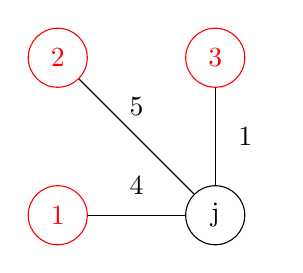
\begin{tikzpicture}[circle, node distance = 2cm, minimum size = 0.75cm]
    \node[draw=red, text=red] (2) {2};
    \node[draw=red, text=red] (3) [right of = 2] {3};
    \node[draw=red, text=red] (1) [below of = 2] {1};
    \node[draw] (j) [below of = 3] {j};

    \path[-] (1) edge node[above] {\(4\)} (j);
    \path[-] (2) edge node[above] {\(5\)} (j);
    \path[-] (3) edge node[right] {\(1\)} (j);
  \end{tikzpicture}
  \caption{Data structure}
  \label{fig:prim-quadratic-data-structure}
  \shortstack{
    nodes \(1, 2, 3 \in S\), node \(j \notin S\) \\
    \(\text{closest}_j = 3 \quad c_{\text{closest}_j j} = 1\)
  }
  \bigskip
\end{figure}

The spanning tree is built is built by selecting the node \(j\) with minimum cost \(C_j\) and adding the edge \(\{j, \textit{closest}_j\}\) to the spanning tree.

\bigskip
The code for this algorithm is shown in Code~\ref{lst:prim-quadratic}.

\begin{lstlisting}[caption={Prim's algorithm in quadratic time}, label={lst:prim-quadratic}, float]
T := {}
S := {u}
// initialization
for j $\notin$ N $\setminus$ S do
  if {u, j} $\in$ E then
    C_j := c_{u, j}
  else
    C_j := +\infty
  end
  closest_j := u
end
for k := 1 to n - 1 do
  min := $+\infty$ // selection of min cost edge
  for j := 1, ..., n do
    if j $\notin$ S and C_j < min then
      min := C_j
      v := j
    end
  end
  S := S $\cup$ {v} // extend S
  T := T $\cup$ {{v, closest_v}} // extend T
  for j := 1 to n do
    if j $\notin$ S and c_vj < C_j then
      C_j := c_vj
      closest_j := v
    end
  end
end
\end{lstlisting}

\bigskip
The complexity of this algorithm is \(\bigO{n^2}\).
For sparse graphs, where \(m \ll \dfrac{n(n-1)}{2}\), a more efficient implementation (\(\bigO{m \log{(n)}}\)) \textit{(using priority queues)} is possible.

\subsubsection{Optimality condition}

Given a spanning tree \(T\), an edge \(e \notin T\) is \textbf{cost decreasing} if when added to \(T\), it creates a cycle \(C\) with \(C \subseteq T \cup \{e\}\) and \(\exists \, f \in C \setminus \{e\} \ \text{such that} \  c_e < c_f\).

\begin{theorem}
  A tree \(T\) is of minimum total cost if and only if no cost decreasing edge exists.
\end{theorem}

\begin{proof}
  \hfill
  \begin{itemize}
    \item[\(\Rightarrow\)] If a \textbf{cost decreasing edge exists}, then \(T\) is \textbf{not of minimum total cost}
    \item[\(\Leftarrow\)] If \textbf{no cost decreasing edge exists}, then \(T\) is \textbf{of minimum total cost}
      \begin{itemize}
        \item let \(T^\ast\) be a minimum cost spanning tree of graph \(G\), found via by Prim's algorithm
        \item it can be verified that \(T^\ast\) can be iteratively \textit{(changing one edge at a time)} transformed into \(T\) without changing the total cost
        \item thus, \(T\) is also optimal
      \end{itemize}
  \end{itemize}

\end{proof}

\subsection{Optimal paths}

\textbf{Optimal} \textit{(shortest, longest, \ldots)} paths have a wide range of applications, including:

\begin{itemize}
  \item \textbf{Google Maps}, \textbf{GPS} navigators
  \item Planning and management of \textbf{transportation}, \textbf{electrical}, and \textbf{telecommunication} \textbf{networks}
  \item \textbf{Problem} planning
\end{itemize}

\bigskip
\begin{problem}[Problem definition]
Given a directed graph \(G = (N, A)\) with a cost \(c_{ij} \in \R\) associated to each arc \((i, j) \in A\), and two nodes \(s\) and \(t\), determine a minimum cost \textit{(shortest)} path from \(s\) to \(t\).
\end{problem}

\begin{itemize}
  \item Each \textbf{value} \(c_{i, j}\) represents the \textbf{cost} \textit{(or length, travel time, \ldots)} of arc \((i, j) \in A\)
  \item Node \(s\) is the \textbf{origin} \textit{(or source)}, node \(t\) is the \textbf{destination} \textit{(or sink)}
\end{itemize}

\begin{property}
  A path \(\langle (i_1, i_2), (i_2, i_3), \ldots, (i_{k-1}, i_k)  \rangle\) is \textbf{simple} if no node is visited more than once
\end{property}

\begin{property}
  If \(c_{ij} \geq 0\) for all \((i, j) \in A\), there is at least one shortest path that is simple.
\end{property}

\subsubsection{Dijkstra's algorithm}

\textbf{Idea}: consider the nodes in increasing order of length \textit{(cost)} of the shortest path from \(s\) to any one of the other nodes.

\bigskip
\textbf{Method}
\begin{itemize}
  \item To each \textbf{node} \(j \in N\), a \textbf{label} \(L_j\) is associated
        \begin{itemize}
          \item[\(\Rightarrow\)] at the end of the algorithm, this label will be the cost of the minimum cost path from \(s\) to \(j\)
        \end{itemize}
  \item Another label \(\textit{predecessor}_j\) is associated to each node \(j \in N\)
        \begin{itemize}
          \item[\(\Rightarrow\)] at the end of the algorithm, this label will be the node that precedes \(j\) on the minimum cost path from \(s\) to \(j\)
        \end{itemize}
  \item Make a \textbf{greedy} choice with respect to the paths from \(s\) to \(j\)
  \item A set of \textbf{shortest paths} from \(s\) to any node \(j \notin s\) can be retrieved backwards from \(t\) to \(s\) iterating over the predecessors
\end{itemize}

\bigskip
\textbf{Goal}
\begin{itemize}[label=\(\rightarrow\)]
  \item \textit{Input}: graph \(G = (N, A)\), cost \(c_{ij} \geq 0 \, \forall \, i, j\), origin \(s \in N\)
  \item \textit{Output}: shortest path from \(s\) to all other nodes in \(G\)
\end{itemize}

\bigskip
\textbf{Data structure}
\begin{itemize}
  \item \(S \subseteq N\): subset of nodes whose labels are permanent
  \item \(X \subseteq N\): subset of nodes with temporary labels
  \item \(L_j = \begin{cases} \text{cost of a shortest path from } s \text{ to } j \quad & j \in S \\ \min\{L_i + c_{ij} \mid   (i, j) \in \delta^+(S) & j \notin S\}\end{cases}\)
        \begin{itemize}[label=\(\rightarrow\)]
          \item given a directed graph \(G\) and the current subset of nodes \(S \subset N\), consider the outgoing cut \(\delta^+(S)\) and select \((u, v) \in \delta^+(S)\) such that: \( L_u + c_{uv} = \min\{L_i + c_{ij} \mid   (i, j) \in \delta^+ (S)\}\)
          \item thus: \(L_u + c_{uv} \leq L_i + c_{ij}, \forall \, (i, j) \in \delta^+(S)\)
        \end{itemize}
  \item \(\text{predecessor}_j = \begin{cases}\text{predecessor of } j \text{ in the shortest path from } s \text{ to } j \quad& j \in S \\ u \text{ such that } L_u + c_{uj} = \min\{L_i + c_{ij} \mid   i \in S\} & j \notin S\end{cases}\)
\end{itemize}

\bigskip
\textbf{Complexity}:
the complexity of the algorithm depends on the how the arc \((u, v)\) is selected among those of the current cut \(\delta^+(u)\).
\begin{itemize}
  \item If all \(m\) arcs are scanned, the overall complexity would be \(\bigO{nm}\), hence \(\bigO{n^3}\)
  \item If all labels \(L_j\) are determined by appropriate updates (as in Prim's algorithm), only a single arc of \(\delta^+(j)\) is scanned, hence the complexity is \(\bigO{n^2}\)
\end{itemize}

\bigskip
\textbf{Notes}:
\begin{itemize}
  \item A set of shortest paths from \(s\) to all the nodes \(j \in N\) can be retrieved backwards from \(t\) to \(s\) iterating over the predecessors
  \item The union of a set of shortest paths from node \(s\) to all the other nodes of \(G\) is an arborescence rooted at \(s\)
  \item Dijkstra's algorithm does not work when there are arcs with negative cost: if \(G\) contains a circuit of negative cost, the shortest path problem may not be well defined
\end{itemize}

\bigskip
The code for this algorithm is shown in Code~\ref{lst:dijkstras-algorithm}.

\begin{lstlisting}[caption={Dijkstra's algorithm}, label={lst:dijkstras-algorithm}, float]
S := {}
X := {s}
for u $\in$ N do
  L_u := $\infty$
end
L_s := 0
while |S| < |N| do
  u := argmin{L_i $|$ i $\in$ X}
  X := X $\backslash$ {u}
  S := S $\cup$ {u}
  for (u, v) $\in \delta^+(\texttt{u})$ do
    if L_v > L_u + c_uv then
      L_v := L_u + c_uv
      predecessor_v := u
      X := X $\cup$ {v}
    end
  end
end
\end{lstlisting}

\paragraph{Correcteness of Dijkstra's algorithm}

\begin{proposition}
  Dijkstra's algorithm is correct.
\end{proposition}

\begin{proof}
  \hfill
  \begin{enumerate}
    \item A the \(k\)-th step:
          \begin{itemize}
            \item \(S = \{s, i_1, \ldots, i_{k-1}\}\)
            \item \(\begin{cases}\text{cost of a minimum cost path from } s \text{ to } j & j \in S \\ \text{cost of a minimum cost path with all intermediate nodes in } S \quad & j \notin S\end{cases}\)
          \end{itemize}
    \item By induction on the number \(k\) of steps:
          \begin{itemize}
            \item base case: for \(k = 1\) the statement holds, since
                  \[S = \{s\}, \quad L_s = 0, \quad L_j = +\infty, \quad \forall \, j \notin S \]
            \item inductive step: assume that the statement holds for \(k+1\)
                  \begin{itemize}
                    \item let \(u \notin S\) be the node that is inserted in \(S\) and \(\phi\) the path from \(s\) to \(u\) such that:
                          \[ L_v + c_{vu} \leq L_i + c_{iu}, \quad \forall \, (i, v) \in \delta^+(S) \]
                    \item every path \(\pi\) from \(s\) to \(u\) has \(c(\pi) \geq c(\phi)\), as there exists \(i \in S\) and \(j \notin S\) such that:
                          \[ \pi = \pi_1 \cup \left\{ \left( i, j \right)  \right\} \cup \pi_2 \]
                          where \((i, j)\) is the first arc in \(\pi \cap \delta^+(S)\)
                    \item it holds that
                          \[ c(\pi) = c(\pi_1) + c_{ij} + c(\pi_2) \geq L_i + c_{ij} \]
                          because \(c_{ij} \geq 0 \Rightarrow c(\pi_2) \geq 0\) and by the choice of \((v, u)\), \(c(\pi_1) \geq L_i\)
                    \item finally, by induction assumption:
                          \[ L_i + c_{ij} \geq L_v + c_{vu} = c(\phi) \]
                    \item a visualization of this step of the proof is shown in Figure~\ref{fig:proof-of-the-induction-step}
                  \end{itemize}
          \end{itemize}
  \end{enumerate}
\end{proof}

\begin{figure}[htbp]
  \centering
  \bigskip
  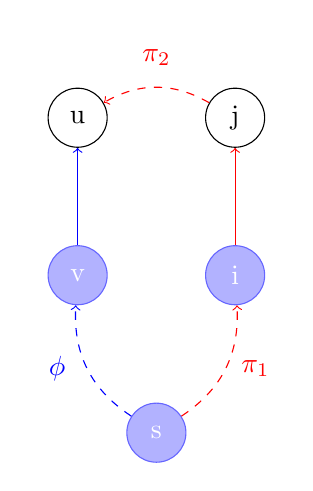
\begin{tikzpicture}[circle, node distance = 2cm, minimum size = 0.75cm]
    \node[draw] (u) at (-2, 0) {u};
    \node[draw] (j) at (0, 0) {j};
    \node[draw=blue!60, text=white, fill=blue!30] (v) at (-2, -2) {v};
    \node[draw=blue!60, text=white, fill=blue!30] (i) at (0, -2) {i};
    \node[draw=blue!60, text=white, fill=blue!30] (s) at (-1, -4) {s};

    \draw[dashed, ->, draw=blue] (s) edge[bend left] node[left, text=blue] {\(\phi\)} (v);
    \draw[dashed, ->, draw=red] (s) edge[bend right] node[right, text=red] {\(\pi_1\)} (i);
    \draw[->, draw=red] (i) edge (j);
    \draw[->, draw=blue] (v) edge (u);
    \draw[dashed, ->, draw=red] (j) edge[bend right] node[above, text=red] {\(\pi_2\)} (u);
  \end{tikzpicture}
  \caption{Proof of the induction step; nodes \(s, v, i\) are in cut \(S\)}
  \label{fig:proof-of-the-induction-step}
  \bigskip
\end{figure}

\paragraph{Example of Dijkstra's algorithm}

An example of Dijkstra's algorithm is shown in Figure~\ref{fig:dijkstra-example}.

\begin{figure}[tbp]
  \centering
  \bigskip
  \begin{subfigure}[t]{\textwidth}
    \centering
    \begin{tikzpicture}[circle, node distance = 2cm, minimum size = 0.75cm]
      \samplegraph

      \path[->] (1) edge node[left=-0.5mm] {5} (2);
      \path[->] (1) edge node[below=-0.5mm] {9} (4);
      \path[->] (2) edge[bend left=15] node[above=-1mm] {3} (3);
      \path[->] (2) edge node[left=-0.5mm] {2} (4);
      \path[->] (3) edge[bend left=15] node[below=-1mm] {1} (2);
      \path[->] (3) edge[bend left=15] node[right=-1mm] {0} (4);
      \path[->] (4) edge[bend left=15] node[left=-1mm] {2} (3);
      \path[->] (3) edge node[above=-0.5mm] {5} (5);
      \path[->] (4) edge node[below=-0.5mm] {9} (5);
    \end{tikzpicture}
    \caption{Sample graph, with the cost of each arc}
  \end{subfigure}
  \bigskip
  \begin{subfigure}[t]{0.32\textwidth}
    \centering
    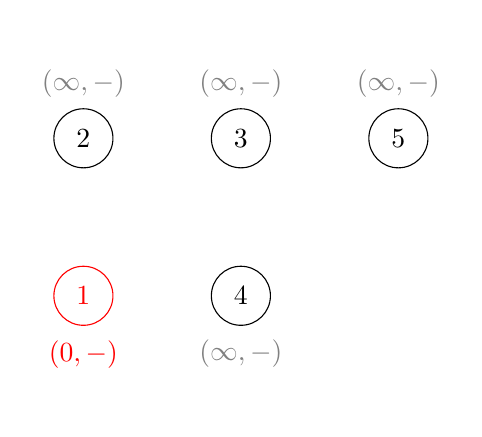
\begin{tikzpicture}[circle, node distance = 2cm, minimum size = 0.75cm]
      \node[draw, label={[text=gray, above=-0.4cm]\((\infty, -)\)}] (2) {2};
      \node[draw, label={[text=gray, above=-0.4cm]\((\infty, -)\)}] (3) [right of = 2] {3};
      \node[draw, label={[text=gray, above=-0.4cm]\((\infty, -)\)}] (5) [right of = 3] {5};
      \node[draw=red, text=red, label={[text=red, below=0.5cm]\((0, -)\)}] (1) [below of = 2] {1};
      \node[draw, label={[text=gray, below=0.4cm]\((\infty, -)\)}] (4) [right of = 1] {4};
    \end{tikzpicture}
    \caption{step 1 of Dijkstra's algorithm}
  \end{subfigure}
  \begin{subfigure}[t]{0.32\textwidth}
    \centering
    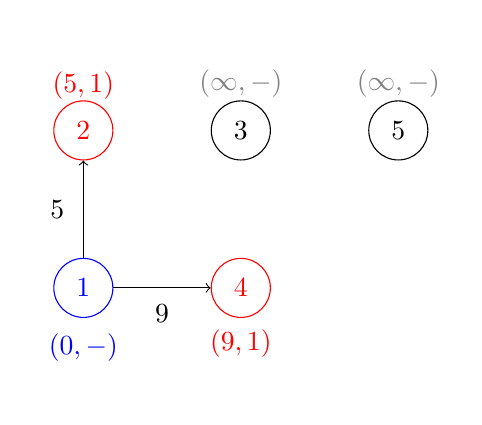
\begin{tikzpicture}[circle, node distance = 2cm, minimum size = 0.75cm]
      \node[draw=red, text=red, label={[text=red, above=-0.4cm]\((5, 1)\)}] (2) {2};
      \node[draw, label={[text=gray, above=-0.5cm]\((\infty, -)\)}] (3) [right of = 2] {3};
      \node[draw, label={[text=gray, above=-0.5cm]\((\infty, -)\)}] (5) [right of = 3] {5};
      \node[draw=blue, text=blue, label={[text=blue, below=0.5cm]\((0, -)\)}] (1) [below of = 2] {1};
      \node[draw=red, text=red, label={[text=red, below=0.5cm]\((9, 1)\)}] (4) [right of = 1] {4};

      \path[->] (1) edge node[left=-0.5mm] {5} (2);
      \path[->] (1) edge node[below=-0.5mm] {9} (4);
    \end{tikzpicture}
    \caption{step 2 of Dijkstra's algorithm}
  \end{subfigure}
  \begin{subfigure}[t]{0.32\textwidth}
    \centering
    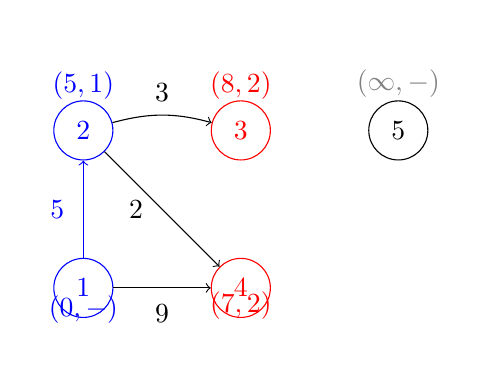
\begin{tikzpicture}[circle, node distance = 2cm, minimum size = 0.75cm]
      \node[draw=blue, text=blue, label={[text=blue, above=-0.4cm]\((5, 1)\)}] (2) {2};
      \node[draw=red, text=red, label={[text=red, above=-0.4cm]\((8, 2)\)}] (3) [right of = 2] {3};
      \node[draw, label={[text=gray, above=-0.5cm]\((\infty, -)\)}] (5) [right of = 3] {5};
      \node[draw=blue, text=blue, label={[text=blue, below = 0.5]\((0, -)\)}] (1) [below of = 2] {1};
      \node[draw=red, text=red, label={[text=red, below = 0.5]\((7, 2)\)}] (4) [right of = 1] {4};

      \path[->, blue] (1) edge node[left=-0.5mm] {5} (2);
      \path[->] (1) edge node[below=-0.5mm] {9} (4);
      \path[->] (2) edge[bend left=15] node[above=-1mm] {3} (3);
      \path[->] (2) edge node[left=-0.5mm] {2} (4);
    \end{tikzpicture}
    \caption{step 3 of Dijkstra's algorithm}
  \end{subfigure}
  \bigskip
  \begin{subfigure}[t]{0.32\textwidth}
    \centering
    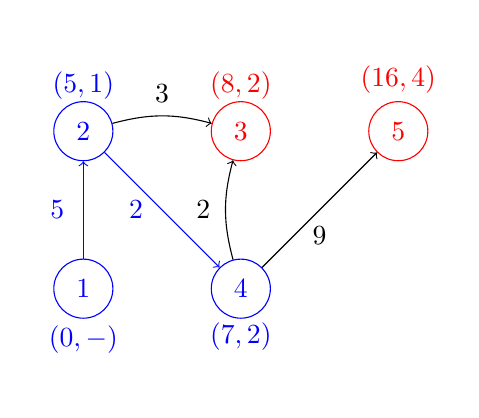
\begin{tikzpicture}[circle, node distance = 2cm, minimum size = 0.75cm]
      \node[draw=blue, text=blue, label={[text=blue, above=-0.4cm]\((5, 1)\)}] (2) {2};
      \node[draw=red, text=red, label={[text=red, above=-0.4cm]\((8, 2)\)}] (3) [right of = 2] {3};
      \node[draw=red, text=red, label={[text=red, above=-0.4cm]\((16, 4)\)}] (5) [right of = 3] {5};
      \node[draw=blue, text=blue, label={[text=blue, below=0.4cm]\((0, -)\)}] (1) [below of = 2] {1};
      \node[draw=blue, text=blue, label={[text=blue, below=0.4cm]\((7, 2)\)}] (4) [right of = 1] {4};

      \path[->, blue] (1) edge node[left=-0.5mm] {5} (2);
      \path[->] (2) edge[bend left=15] node[above=-1mm] {3} (3);
      \path[->, blue] (2) edge node[left=-0.5mm] {2} (4);
      \path[->] (4) edge[bend left=15] node[left=-1mm] {2} (3);
      \path[->] (4) edge node[below=-0.5mm] {9} (5);
    \end{tikzpicture}
    \caption{step 4 of Dijkstra's algorithm}
  \end{subfigure}
  \begin{subfigure}[t]{0.32\textwidth}
    \centering
    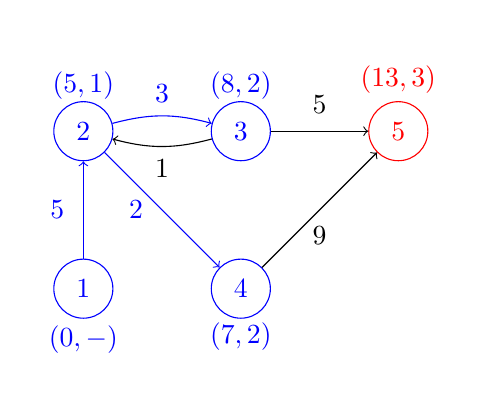
\begin{tikzpicture}[circle, node distance = 2cm, minimum size = 0.75cm]
      \node[draw=blue, text=blue, label={[text=blue, above=-0.4cm]\((5, 1)\)}] (2) {2};
      \node[draw=blue, text=blue, label={[text=blue, above=-0.4cm]\((8, 2)\)}] (3) [right of = 2] {3};
      \node[draw=red, text=red, label={[text=red, above=-0.4cm]\((13, 3)\)}] (5) [right of = 3] {5};
      \node[draw=blue, text=blue, label={[text=blue, below=0.4cm]\((0, -)\)}] (1) [below of = 2] {1};
      \node[draw=blue, text=blue, label={[text=blue, below=0.4cm]\((7, 2)\)}] (4) [right of = 1] {4};

      \path[->, blue] (1) edge node[left=-0.5mm] {5} (2);
      \path[->, blue] (2) edge[bend left=15] node[above=-1mm] {3} (3);
      \path[->, blue] (2) edge node[left=-0.5mm] {2} (4);
      \path[->] (3) edge[bend left=15] node[below=-1mm] {1} (2);
      \path[->] (3) edge node[above=-0.5mm] {5} (5);
      \path[->] (4) edge node[below=-0.5mm] {9} (5);
    \end{tikzpicture}
    \caption{step 5 of Dijkstra's algorithm}
  \end{subfigure}
  \begin{subfigure}[t]{0.32\textwidth}
    \centering
    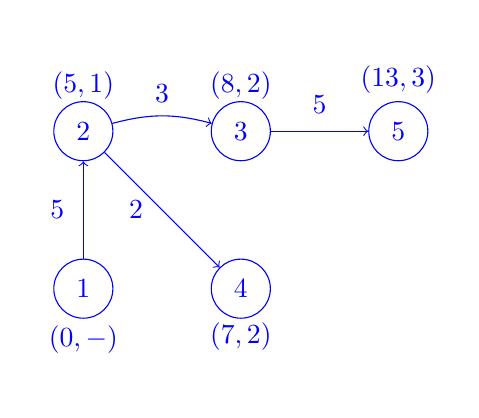
\begin{tikzpicture}[circle, node distance = 2cm, minimum size = 0.75cm]
      \node[draw=blue, text=blue, label={[text=blue, above=-0.4cm]\((5, 1)\)}] (2) {2};
      \node[draw=blue, text=blue, label={[text=blue, above=-0.4cm]\((8, 2)\)}] (3) [right of = 2] {3};
      \node[draw=blue, text=blue, label={[text=blue, above=-0.4cm]\((13, 3)\)}] (5) [right of = 3] {5};
      \node[draw=blue, text=blue, label={[text=blue, below=0.4cm]\((0, -)\)}] (1) [below of = 2] {1};
      \node[draw=blue, text=blue, label={[text=blue, below=0.4cm]\((7, 2)\)}] (4) [right of = 1] {4};

      \path[->, blue] (1) edge node[left=-0.5mm] {5} (2);
      \path[->, blue] (2) edge[bend left=15] node[above=-1mm] {3} (3);
      \path[->, blue] (2) edge node[left=-0.5mm] {2} (4);
      \path[->, blue] (3) edge node[above=-0.5mm] {5} (5);
    \end{tikzpicture}
    \caption{step 6 of Dijkstra's algorithm}
  \end{subfigure}
  \caption{Example of Dijkstra's algorithm}
  \label{fig:dijkstra-example}
\end{figure}

\subsubsection{Floyd-Warshall's algorithm}

\textbf{Goal}
\begin{itemize}[label=\(\rightarrow\)]
  \item \textit{Input}: a directed graph \(G = (N, A)\) with an \(n \times n\) cost matrix \(C = [c_{ij}]\)
  \item \textit{Output}: for each pair of nodes \(i, j \in N\), the cost \(c_{ij}\) of the shortest path from \(i\) to \(j\)
\end{itemize}

\bigskip
\textbf{Data structure}
\begin{itemize}
  \item Two \(n \times n\) matrices \(D, P\) whose elements correspond, at the end of the algorithm, to:
        \begin{itemize}
          \item[\(d_{ij}\)] the cost of the shortest path from \(i\) to \(j\)
          \item[\(p_{ij}\)] the predecessor of \(j\) on the shortest path from \(i\) to \(j\)
        \end{itemize}
\end{itemize}

\bigskip
\textbf{Method}
\begin{enumerate}
  \item Initialization of \(D\) and \(P\):
        \[ p_{ij} = i \quad \forall \, i \]
        \[ d_{ij} = \begin{cases} 0 \quad & i = j \\ c_{ij} & i \neq j \land (i, j) \in A \\ +\infty & \text{otherwise}  \end{cases} \]
  \item Triangular operation: for each pair of nodes \(i, j\), where \(i \neq u, j \neq u\), check whether the path from \(i\) to \(j\) is shorter by going through \(u\) (i.e. \(d_{iu} + d_{uj} < d_{ij}\))
\end{enumerate}

\bigskip
\textbf{Complexity}
\begin{itemize}
  \item Since in the worst case the triangular operation is executed for all nodes \(u\) ad for each pair of nodes \(i, j\), the complexity is \(\bigO{n^3}\)
\end{itemize}

\bigskip
The code for this algorithm is shown in Code~\ref{lst:floyd-warshall-algorithm}.

\begin{lstlisting}[caption={Floyd-Warshall's algorithm}, label={lst:floyd-warshall-algorithm}, float]
for j := 1 to n do
  p_id := i

  if i = j then
    d_ij := 0
  else if (i, j) in A then
    d_ij := c_ij
  else
    d_ij := $+\infty$
  end
end
for u $\in$ N do
  for i $\in$ N $\setminus\{$ u $\}$ do
    for j $\in$ N $\setminus\{$ u $\}$
      if d_iu + d_uj < d_ij then
        p_ij := p_uj
        d_ij := d_iu + d_uj
      end
    end
  for i $\in$ N do
    if d_ij < 0 then
      error "negative cycle"
    end
  end
end
\end{lstlisting}

\paragraph{Correctness of Floyd-Warshall's algorithm}

\begin{proposition}
  Floyd-Warshall's algorithm is correct.
\end{proposition}

\begin{proof}
  assume that the nodes of \(G\) are numbered from \(1\) to \(n\).
  Verify that, if the node index order is followed, after the \(u\)-th cycle the value \(d_{ij}\) \textit{(for any \(i, j\))} corresponds to the cost of a shortest path from \(i\) to \(j\) with at most \(u\) intermediate nodes (\(\left\{ 1, \ldots, u \right\}\))
\end{proof}

\subsection{Optimal paths in directed, acyclic graphs}

A directed graph \(G = (N, A)\) is \textbf{acyclic} if it does not contain any circuit.
A directed acyclic graph \(G\) is referred to as a \DAG.

\begin{property}[topological ordering]
  The nodes of any \DAG \(G\) can be ordered topologically, i.e. indexed so that for each arc \((i, j) \in A\) the index of \(i\) is less than the index of \(j\) \textit{(\(i \leq j\))}.
\end{property}

The topological order can be exploited by dynamic programming algorithms to compute efficiently the shortest paths in a \DAG.

\begin{problem}[Problem description]
  Given a \DAG \(G = (N, A)\) with a cost \(c_{ij} \in \R\) and nodes \(s, t\), determine the shortest (or longest) path from \(s\) to \(t\).
\end{problem}

\subsubsection{Topological ordering method}

The method requires \(G = (N, A)\) to be a \DAG represented via the list of predecessors \(\delta^-(v)\) and the list of successors \(\delta^+(v)\) of each node \(v \in N\).
Then, it works as follows:

\begin{enumerate}[label=\arabic*., ref=(\arabic*)]
  \item\label{enum:topological-ordering-1} Assign the smallest positive integer not yet assigned to a node \(v \in N \) with \(\delta^-(v) = \emptyset\)
  \begin{itemize}[label=\(\rightarrow\)]
    \item such node always exists because \(G\) does not contain circuits
  \end{itemize}
  \item Delete the node \(v\) with all its incident arcs
  \item Go to step  \ref{enum:topological-ordering-1} until all nodes have been assigned a number
\end{enumerate}

\begin{figure}[htbp]
  \centering
  \bigskip
  \begin{subfigure}[t]{0.495\textwidth}
    \centering
    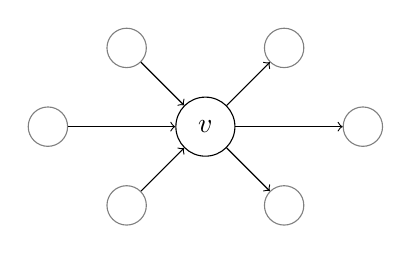
\begin{tikzpicture}[circle]
      \node[draw, circle, minimum size=0.75cm] (v) at (0, 0) {\(v\)};
      \node[draw=gray,circle, minimum size=0.5cm] (0) at (-1, -1) {};
      \node[draw=gray,circle, minimum size=0.5cm] (1) at (-2, 0) {};
      \node[draw=gray,circle, minimum size=0.5cm] (2) at (-1, 1) {};
      \node[draw=gray,circle, minimum size=0.5cm] (3) at (1, -1) {};
      \node[draw=gray,circle, minimum size=0.5cm] (4) at (2, 0) {};
      \node[draw=gray,circle, minimum size=0.5cm] (5) at (1, 1) {};

      \draw[->] (0) -- (v);
      \draw[->] (1) -- (v);
      \draw[->] (2) -- (v);

      \draw[->] (v) -- (3);
      \draw[->] (v) -- (4);
      \draw[->] (v) -- (5);
    \end{tikzpicture}
    \caption{Topological ordering}
    \label{fig:topological-ordering}
  \end{subfigure}
  \begin{subfigure}[t]{0.495\textwidth}
    \centering
    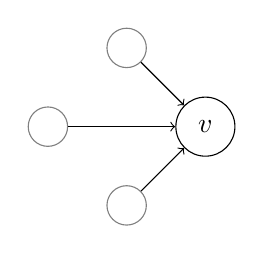
\begin{tikzpicture}[circle]
      \node[draw, circle, minimum size=0.75cm] (v) at (0, 0) {\(v\)};
      \node[draw=gray,circle, minimum size=0.5cm] (0) at (-1, -1) {};
      \node[draw=gray,circle, minimum size=0.5cm] (1) at (-2, 0) {};
      \node[draw=gray,circle, minimum size=0.5cm] (2) at (-1, 1) {};

      \draw[->] (0) -- (v);
      \draw[->] (1) -- (v);
      \draw[->] (2) -- (v);
    \end{tikzpicture}
    \caption{Node \(v\) with \(\delta^-(v) = \emptyset\), as in step \ref{enum:topological-ordering-1} of the algorithm}
    \label{fig:node-with-empty-successors}
  \end{subfigure}
  \caption{Topological ordering method}
  \label{fig:topological-ordering-method}
  \bigskip
\end{figure}

\bigskip
This algorithm has complexity \(\bigO{|A|}\), because each node is assigned a number only once.
Furthermore, all arcs incident to a node are deleted only once.

\subsubsection{Dynamic programming for shortest path in \DAGs}

Any shortest path from \(1\) to \(t\), called \(\pi_t\), with at least \(2\) arcs can be subdivided into two parts:

\begin{itemize}
  \item \(\pi_i\), the shortest subpath from \(s\) to \(i\)
  \item \(\left( i, t \right)\), the remaining part
\end{itemize}

This decomposition is called the optimality principle of shortest paths in \DAGs.
An illustration of this decomposition is shown in Figure \ref{fig:shortest-path-in-DAG}.

\begin{figure}[htbp]
  \centering
  \bigskip
  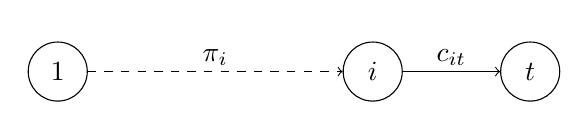
\begin{tikzpicture}[circle, minimum size = 0.75cm]
    \node[draw, circle] (1) at (-1, 0) {\(1\)};
    \node[draw, circle] (i) at (3, 0) {\(i\)};
    \node[draw, circle] (t) at (5, 0) {\(t\)};

    \draw[] (1) edge[dashed, ->] node[above=-0.2cm] {\(\pi_i\)} (i);
    \draw[->] (i) edge node[above=-0.2cm] {\(c_{it}\)} (t);
  \end{tikzpicture}
  \caption{Shortest path from \(1\) to \(t\)}
  \label{fig:shortest-path-in-DAG}
  \bigskip
\end{figure}

\bigskip
The strategy to find the shortest path is:

\begin{enumerate}
  \item For each node \(i = 1, \ldots, t\) let \(L_i\) be the cost of a shortest path from \(1\) to \(i\)
        \begin{itemize}[label=\(\rightarrow\)]
          \item \(L_t = \displaystyle \min_{(i, t) \in \delta^-(t)} \left\{ L_i + c_{it} \right\}\)
          \item the minimum is taken over all possible predecessors \(i\) of \(t\)
        \end{itemize}
  \item If \(G\) is topologically ordered \DAG, then the only possible predecessors of \(t\) in a shortest path \(\pi_t\) from \(1\) to \(t\) are those with index \(i < t\)
        \begin{itemize}[label=\(\rightarrow\)]
          \item \(L_t = \displaystyle \min_{i < t} \left\{ L_i + c_{it} \right\}\)
          \item in a graph with circuits, any node \(i\) can be a predecessor of \(t\) if \(i \neq t\)
        \end{itemize}
\end{enumerate}

For \DAGs whose nodes are topologically ordered \(L_{t-1}, \ldots, L_1\) satisfy the same type of recursive relations:

\[ L_{t-1} = \displaystyle \min_{i < t-1} \left\{ L_i + c_{i, t-1} \right\}; \ldots; L_2 = \displaystyle \min_{i=1}\left\{ L_i + c_{i2} \right\} = L_1 + c_{12}; L_1 = 0 \]
which can be solved in reversed order
\[ L_1 = 0; L_2 = L_1 + c_{12}; \ldots; L_{t} = \displaystyle \min_{i < t - 1} \left\{ L_i + c_t \right\} \]

\bigskip
\textbf{Algorithm}:
finally, the algorithm is shown in pseudocode in Code~\ref{lst:shortest-path-in-DAG}.

\begin{lstlisting}[caption={Shortest path in \DAG}, label={lst:shortest-path-in-DAG}, float]
sort the nodes of G topologically
L_1 := 0
for j := 2 to n do
  L_j := min{L_i + c_{ij} | (i, j) $\in \delta^-(\texttt{j})\ \land\ \texttt{i} < \texttt{j}$}
  pred_j := v such that (v, j) = argmin{L_i + c_{ij} | (i, j) $\in \delta^-(\texttt{j})\ \land\ \texttt{i} < \texttt{j}$}
end
\end{lstlisting}

\bigskip
\textbf{Complexity}
of the algorithm is \(\bigO{|A|}\):

\begin{itemize}
  \item Topological ordering of the nodes: \(\bigO{m}\) with \(m = |A|\) \textit{(number of arcs)}
  \item Each node/arc is processed only once: \(\bigO{n+m}\)
\end{itemize}

\bigskip
In order to find the longest path, the algorithm can be adapted as follows:
\[L_t = \displaystyle \max_{i < t} \left\{ L_i + c_{it} \right\}\]

\paragraph{Optimality of the algorithm}

The Dynamic Programming algorithm for finding shortest or longest paths in \DAGs is exact.
This is due to the optimality principle, already explored in the previous section.

\subsection{Project planning}

\begin{problem}[Problem definition]
A project consists of a set of \(m\) activities with their (estimated) duration: activity \(A_i\) has duration \(d_i \geq 0, i = 1, \ldots, m\).
Some pair of activities allow a precedent constraint: \(A_i \propto A_j\) indicated that \(A_i\) must be performed before \(A_j\).

A project can be represented by a directed graph \(G = (N, A)\) where:
\begin{itemize}
  \item each arc corresponds to an activity
  \item the arc length represent the duration of the corresponding activity
\end{itemize}
\end{problem}

\bigskip

In order to account for precedence constraints, the arcs must be positioned such that for activities \(A_i \propto A_j\) there exists a directed path where the arc associated to \(A_i\) precedes the arc associated to \(A_j\).
Such notation is shown in Figure \ref{fig:precedence-relation-in-project-planning}.

\begin{figure}[htbp]
  \centering
  \bigskip
  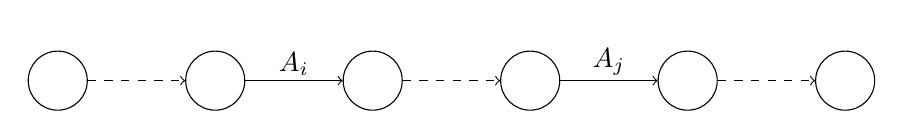
\begin{tikzpicture}[circle, node distance = 2cm, minimum size = 0.75cm]
    \node[draw] (1) {};
    \node[draw] (2) [right of = 1] {};
    \node[draw] (3) [right of = 2] {};
    \node[draw] (4) [right of = 3] {};
    \node[draw] (5) [right of = 4] {};
    \node[draw] (6) [right of = 5] {};

    \draw[dashed, ->] (1) edge (2);
    \draw[->] (2) edge node[above=-0.2cm]{\(A_i\)} (3);
    \draw[dashed, ->] (3) edge (4);
    \draw[->] (4) edge node[above=-0.2cm]{\(A_j\)} (5);
    \draw[dashed, ->] (5) edge (6);
  \end{tikzpicture}
  \bigskip
  \caption{Precedence relation in project planning}
  \label{fig:precedence-relation-in-project-planning}
\end{figure}

Therefore, a nove \(v\) marks an event corresponding to the end fo all the activities \(\left( i, v \right) \in \delta^-(v)\) and the \textit{(possible)} start of all the activities \(\left( v, j \right) \in \delta^+(v)\).

\bigskip

\begin{property}
  The directed graph \(G\) representing a project is acyclic \textit{(is a \DAG)}.
\end{property}

\begin{proof}
  by contradiction, if \(A_{i1} \propto A_{12} \propto \ldots \propto A_{jk} \propto A_{kj}\) there would be a logical inconsistency.
\end{proof}

\subsubsection{Optimal paths}

A graph \(G\) can be simplified by contracting some arcs, but it's important to not introduce unwanted precedence constraints.
Artificial nodes or artificial arcs are introduced so that graph \(G\):

\begin{itemize}
  \item Contains a \textbf{unique initial node} \(s\) corresponding to the event \inlinequote{beginning of the project}
  \item Contains a \textbf{unique final node} \(t\) corresponding to the event \inlinequote{end of the project}
  \item Does not contain \textbf{multiple arcs} with the \textbf{same origin and destination}
\end{itemize}

\bigskip
\begin{problem}[Problem description]
  Given a project (set of activities with duration and precedence constraints), schedule the activities in order to minimize the overall project duration (the time needed to complete all the activities).
\end{problem}

\bigskip
\begin{property}
  The minimum overall project duration is the length of a longest path from \(s\) to \(t\) in the graph \(G\).
\end{property}

\begin{proof}
  since any \(s-t\) path represents a sequence of activities that must be executed in the specified order, its length provides a lower bound on the minimum overall project duration.
\end{proof}

\paragraph{Critical path method - \CPM}

The critical path method \textit{(\CPM) } determines:

\begin{itemize}
  \item A \textbf{schedule} \textit{(a plan for executing the activities specifying the order and the assigned time)} that minimizes the overall project duration
  \item The \textbf{slack} of each activity \textit{(the amount of time by which its execution can be delayed without affecting the overall minimum project duration)}
\end{itemize}

\bigskip
\textbf{Initialization}
construct the graph \(G\) representing the project.

\bigskip
\textbf{Method}

\begin{enumerate}
  \item Find a topological order of the nodes
  \item Consider the nodes by increasing indices and for each \(h \in N\) find the earliest time \(T_{min_h}\) at which the event associated to node \(h\) can occur
        \begin{itemize}[label = \(\rightarrow\)]
          \item \(T_{min_h}\) corresponds to the minimum project duration
        \end{itemize}
  \item Consider the nodes by decreasing indices and for each \(h \in N\) find the latest time \(T_{max_h}\) at which the event associated to node \(h\) can occur without delaying the project completion date beyond \(T_{min_n}\)
  \item For each activity \(\left( i, j \right) \in A\) find the slack
        \begin{itemize}[label = \(\rightarrow\)]
          \item the slack is calculated as \(\sigma{ij} = T_{max_j} - T_{min_i} - d_{ij}\)
        \end{itemize}
\end{enumerate}

\bigskip
\textbf{Goal}
\begin{itemize}[label=\(\rightarrow\)]
  \item \textit{Input:} graph \(G = (N, A)\) with \(n = |N|\) and the duration \(d_{ij}\) associated to each \(\left( i, j \right) \in A\)
  \item \textit{Output}: \(\left( T_{min_i}, T_{max_i} \right), i = 1, \ldots, n\)
\end{itemize}

\bigskip
\textbf{Algorithm}:
finally, the algorithm is shown in pseudocode in Code~\ref{lst:critical-path-method}.

\begin{lstlisting}[caption={Critical path method}, label={lst:critical-path-method}, float]
sort the nodes topologically
T_min_i := 0
for j = 2 to n do
  T_min_j := max{T_min_i + d_ij | (i, j) $\in \delta^- (\texttt{j})$}
end
T_max_n := T_min_n // minimum project duration
for i = n-1 to 1 do
  T_max_i := min{T_max_j - d_ij | (i, j) $\in \delta^+ (\texttt{i})$}
end
\end{lstlisting}

\bigskip
\textbf{Complexity}:
the overall complexity is \(\bigO{n+m} \approx \bigO{m}\), due to the sum of

\begin{itemize}
  \item complexity of the topological sort - \(\bigO{n+m}\)
  \item complexity of the first loop - \(\bigO{n+m}\)
  \item complexity of the second loop - \(\bigO{n+m}\)
\end{itemize}

\paragraph{Critical paths}

An activity \(\left( i, j \right)\) with zero slack \(\sigma_{ij} = T_{max_j} = T_{min_i} = d_{ij} = 0\) is called \textbf{critical}.

A critical path is a path in a \(s-t\) composed uniquely by critical activities.
At least one always exists.

\paragraph{Gantt charts}

A Gantt chart is a graphical representation of a project schedule.
It was introduced in 1896 by Henry Gantt, an American mechanical engineer and management consultant.

There are two types of Gantt charts:

\begin{itemize}
  \item Gantt chart at \textbf{earliest} - each activity \(\left( i, j \right)\) starts at \(T_{min_i}\) and ends at \(T_{min_i} + d_{ij}\)
  \item Gantt chart at \textbf{latest} - each activity \(\left( i, j \right)\) starts at \(T_{max_i}\) and ends at \(T_{max_i} + d_{ij}\)
\end{itemize}

\subsection{Network flows}

Network flows problems involve the distribution of a given \textit{product} \textit{(such as water, gas, data)} from a set of \textit{sources} to a set of \textit{users} so as to optimize a given objective function \textit{(e.g. minimize the total cost of the distribution)}.

It has many indirect applications, such as:

\begin{itemize}
  \item \textbf{Telecommunication}
  \item \textbf{Transportation}
  \item \textbf{Logistics}
\end{itemize}

\begin{itemize}
  \item A \textbf{network} is a directed and connected graph \(G = (V, A)\) with a source \(s \in V\) and a sing \(t \in V\), with \(s \neq t\), and a capacity \(k_{ij} \geq 0\) for each arc \((i, j) \in A\).
  \item A \textbf{feasible flow} \(x\) from \(s\) to \(t\) is a vector \(x \in \R^m\) with a component \(x_{ij}\) for each arc \((i, j) \in A\) satisfying the capacity constraint \[0 \leq x_{ij} \leq k_{ij}, \quad \forall \, \left( i, j \right) \in A\]
        and the flow balance constraint at each intermediate node \(u \in \left\{ V \setminus \{s, t\} \right\}\):
        \[\displaystyle \sum_{\left( i, u \right) \in \delta^{-}(u)} x_{iu} = \displaystyle \sum_{\left( u, j \right) \in \delta^{+}(u)} x_{uj} \quad \forall \, u \in N \setminus \left\{ s, t \right\} \]
  \item The value of \textbf{flow} \(x\) is \(\phi = \displaystyle \sum_{\left( s, j \right) \in \delta^{+}(s)} x_{sj}\)
  \item Given a network and a feasible flow \(x\), an arc \(\left( i, j \right) \in A\) is \textbf{saturated} if \(x_{ij} = k_{ij}\) and \textbf{empty} if \(x_{ij} = 0\)
\end{itemize}

\bigskip
A problem related to flow is defined as follows \textit{(Definition~\ref{def:flow-problem})}.
\begin{definition}[flow Problem definition]
  Given a network \(G = \left( V, A \right)\) with an integer capacity \(k_{ij}\) for each arc \((i, j) \in A\), find a feasible flow \(x\) from \(s\) to \(t\) with maximum value.

  If multiple sources or sink are present while only one product is considered, dummy notes \(s^\ast\) and \(t^\ast\) can be added \textit{(as shown in Figure~\ref{fig:multiple-sources-sinks})}.
  \label{def:flow-problem}
\end{definition}

\begin{figure}[htbp]
  \centering
  \bigskip
  \
  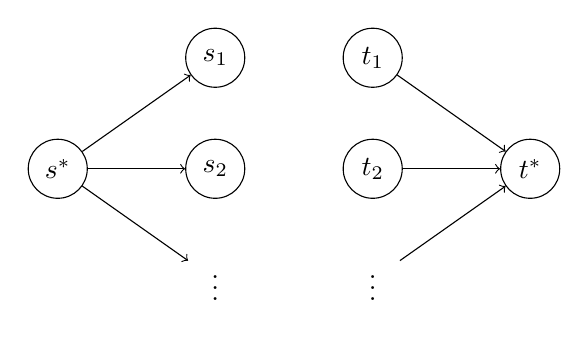
\begin{tikzpicture}[circle, minimum size = 0.75cm]
    \node[draw] (s) at (0, 0) {\(s^\ast\)};
    \node[draw] (s1) at (2, 1.41) {\(s_1\)};
    \node[draw] (s2) at (2, 0) {\(s_2\)};
    \node[] (s3) at (2, -1.41) {\vdots};

    \node[draw] (t1)  at (4, 1.41) {\(t_1\)};
    \node[draw] (t2)  at (4, 0) {\(t_2\)};
    \node[] (t3)  at (4, -1.41) {\vdots};
    \node[draw] (t) at (6, 0) {\(t^\ast\)};

    \path[->] (s) edge (s1);
    \path[->] (s) edge (s2);
    \path[->] (s) edge (s3);

    \path[->] (t1) edge (t);
    \path[->] (t2) edge (t);
    \path[->] (t3) edge (t);
  \end{tikzpicture}
  \caption{Multiple sources and sinks. \(\delta^-(s^\ast) = \delta^+(t^\ast) = \emptyset\), \(k_{s^\ast i} = \text{availability limit}\), \(k_{jt^\ast} = \infty\)}
  \label{fig:multiple-sources-sinks}
  \bigskip
\end{figure}
\begin{figure}[htbp]
  \centering
  \bigskip
  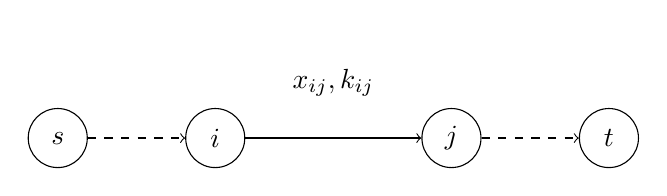
\begin{tikzpicture}[circle, minimum size = 0.75cm]
    \node[draw] (s) at (0, 0) {\(s\)};
    \node[draw] (i) at (2, 0) {\(i\)};
    \node[draw] (j) at (5, 0) {\(j\)};
    \node[draw] (t) at (7, 0) {\(t\)};

    \path[->, dashed] (s) edge (i);
    \path[->] (i) edge node[above] {\(x_{ij}, k_{ij}\)} (j);
    \path[->, dashed] (j) edge (t);
  \end{tikzpicture}
  \caption{Graph representation of a flow}
  \label{fig:flow-graph-representation}
  \bigskip
\end{figure}

\subsubsection{Linear programming model}

The linear programming model \textit{(refer to Section~\ref{sec:linear-programming} for a in dept explanation of linear programming)} of the network flow is defined as:

\begin{gather*}
  \begin{aligned}
    \max \quad        & \phi                                                                                                                                                                                       \\
    \text{s.t.} \quad & \displaystyle \sum_{\left( u, j \right) \in \delta^+(u)} x_{uj} + \displaystyle \sum_{\left( i, u \right) \in \delta^-(u)} x_{iu} & = \begin{cases}
                                                                                                                                                                \phi \quad   & \text{if } u = s \\
                                                                                                                                                                - \phi \quad & \text{if } u = t \\
                                                                                                                                                                0 \quad      & \text{otherwise}
                                                                                                                                                              \end{cases} \\
                      & 0 \leq x_{ij} \leq k_{ij} \quad \forall \, \left( i, j \right) \in A                                                                                                                       \\
                      & \phi \in \R, x_{ij} \in \R \quad \forall \, \left( i, j \right) \in A
  \end{aligned}
\end{gather*}

where \(\phi\) denotes the value of the \textbf{feasible flow} \(x\);
\(\phi\) is also the amount of product extracted from the source \(s\).

\begin{itemize}
  \item A \textbf{cut} separating \(s\) from \(t\) is \(\delta(S) \text{ of } G, \ s \in S, \ t \in V \setminus S\)
  \item There are \(2^{n-2}\) cuts from \(s\) to \(t\), with \(n = |V|\)
  \item The \textbf{capacity} of the cut \(\delta(S)\) induced by \(S\) is: \[ k(S) = \displaystyle \sum_{\left( i, j \right) \in \delta^+(S)} k_{ij} \]
  \item Given a feasible flow \(x\) from \(s\) to \(t\) and a cut \(\delta(S)\) separating them, the value of the \textbf{feasible flow through the cut} is \[\phi(S) = \displaystyle \sum_{\left( i, j \right) \in \delta^+(S)} x_{ij} - \sum_{\left( i, j \right) \in \delta^-(S)} x_{ij}\]
        with this notation, the value of the flow \(x\) is \(\phi = \phi\left( \left\{ s \right\} \right)\)
\end{itemize}

\subsubsection{Properties of the flows}
\begin{property}
  Given a feasible flow \(x\) from \(s\) to \(t\), for each cut separating \(\delta(S)\) separating \(s\) from \(t\):
  \[ \phi(S) = \phi\left( \left\{ s \right\} \right) \]

  This Property is implied by the flow balance equations \(\forall \, v \ \in V \setminus \left\{ s, t \right\}\).
\end{property}

\bigskip
\begin{property}[weak duality]
  For every feasible flow \(s\) from \(s\) to \(t\) and every cut \(\delta(S), \ s \in V\) separating \(s\) from \(t\):
  \[ \phi(s) \leq k(S) \quad \left( \text{value of the flow } \leq \text{ capacity of the cut} \right)\]
  \label{prop:weak-duality}
\end{property}
\begin{proof}
  By definition of value of the flow through the cut \(\delta(S\):
  \[ \phi(S) = \displaystyle \sum_{\left( i, j \right) \in \delta^+(S)} x_{ij} - \sum_{\left( i, j \right) \in \delta^-(S)} x_{ij} \]
  And, since \(0 \leq x_{ij} \leq k_{ij}\) for all \(\left( i, j \right) \in A\):
  \[ \displaystyle \sum_{\left( i, j \right) \in \delta^+(S)} x_{ij} - \sum_{\left( i, j \right) \in \delta^-(S)} x_{ij} \leq \displaystyle \sum_{\left( i, j \right) \in \delta^+(S)} k_{ij} = k(s) \]
  Finally, \(\phi(S) \leq k(S)\).
\end{proof}

\textbf{Consequence:}
If \(\phi(S) = k(S)\), for a subset \(S \subseteq V, \ s \in S, \ t \notin S\), then \(x\) is a flow of maximum value and the cut \(\delta(S)\) is of minimum capacity.

The property \textit{(\ref{prop:weak-duality})} for any feasible flow \(x\) and for any cut \(\delta(S)\) separating \(s\) from \(t\) expresses a \textbf{weak duality relation} between the two problems of finding a maximum flow and a minimum cut.

\begin{itemize}
  \item \textbf{Primal problem}: given \(G = (V, A)\) with integer capacities on the arcs and \(s, t \in V\), determine a feasible flow of maximum problem
  \item \textbf{Dual problem}: given \(G = (V, A)\) with integer capacities on the arcs and \(s, t \in V\), determine a cut \textit{(separating \(s\) from \(t\))} of minimum capacity separating \(s\) from \(t\)
\end{itemize}

\subsubsection{Ford-Fulkerson algorithm}

\textbf{Idea}
start from a feasible flow \(x\) and try to iteratively increase its value \(\phi\) by sending, at each iteration, an additional amount of product along a directed \textit{(or undirected)} path from \(s\) to \(t\) with a strictly positive residual capacity.

\begin{itemize}
  \item If \(\left( i, j \right)\) is not saturated (i.e. \(x_{ij} < k_{ij}\)), then \(\left( i, j \right)\) is called a \textbf{residual arc} and \(x_{ij}\) can be increased
  \item If \(\left( i, j \right)\) is not empty (i.e. \(x_{ij} \geq 0\)), then \(\left( i, j \right)\) is called a \textbf{reverse arc} and \(x_{ij}\) can be decreased while respecting the flow balance equations
\end{itemize}

\bigskip
An arc \(\left( i, j \right)\) in a \(s-t\) cut, where \(s \in S,\ t \in S^\prime\), is called:
\begin{itemize}
  \item \textbf{forward} if \(s \in S, t \in S^\prime\)
  \item \textbf{backward} if \(s \in S^\prime, t \in S\)
\end{itemize}

The following Property (\ref{prop:augmenting-path}) is the key to the Ford-Fulkerson algorithm.
\begin{property}[augmenting path]
  A path \(P\) from \(s\) to \(t\) is an \textbf{augmenting path} with respect to the current feasible flow \(x\) if \(x_{ij} <k_{ij}\) for any forward arc and \(x_{ij} > 0\) for any backward arc.
  \label{prop:augmenting-path}
\end{property}

Then the algorithm works by sending \(\delta\) additional units of product can be sent from \(s\) to \(t\):

\begin{itemize}
  \item \(+\delta\) along forward arcs
  \item \(-\delta\) along backward arcs
\end{itemize}

\bigskip
Given a feasible flow \(x\) for \(G = (V, A)\), a \textbf{residual network} \(\overline{G} = (V \overline{A})\) associated to \(x\) is defined as follows:

\begin{itemize}
  \item If \(\left( i, j \right) \in A\) is not empty, \(\left( j, i \right) \in \overline{A}\) with \(\overline{k}_{ij} = x_{ij} > 0\)
  \item If \(\left( i, j \right) \in A\) is not saturated, \(\left( i, j \right) \in \overline{A}\) with \(\overline{k}_{ij} = k_{ij} - x_{ij} > 0\)
        \begin{itemize}[label=\(\rightarrow\)]
          \item \(\overline{k}_{ij}\) is called the \textbf{residual capacity} of \(\left( i, j \right)\)
        \end{itemize}
\end{itemize}

At each iteration:

\begin{itemize}
  \item Find an augmenting path \(P\) from \(s\) to \(t\)
  \item Send \(\delta\) units of product along \(P\)
  \item Update the feasible flow \(x\) and the residual network \(\overline{G}\)
\end{itemize}

\bigskip
\textbf{Goal}
\begin{itemize}[label=\(\rightarrow\)]
  \item \textit{Input}: graph \(G = (N. A)\) with capacity \(k_{ij} > 0\) for any \((i, j) \in A, \ s,t \in N\)
  \item \textit{Output}: a feasible flow \(x\) from \(s\) to \(t\) of maximum value \(\phi^\ast\)
\end{itemize}

The pseudocode is shown in Code~\ref{code:ford-fulkerson}.

\begin{lstlisting}[caption={Ford-Fulkerson algorithm}, label={code:ford-fulkerson}]
x := 0
phi := 0
optimum := false
do
  build residual network $\overline{\texttt{G}}$ associated to x
  P := path from s to t in $\overline{\texttt{G}}$
  if P is not defined then
    optimum := true
  else
    delta := min residual capacity of arcs in P
    phi := phi + delta
    for each arc (i, j) in P do
      if (i, j) is a forward arc then
        $\texttt{x}_{\texttt{ij}}$ := $\texttt{x}_{\texttt{ij}}$ + delta
      else
        $\texttt{x}_{\texttt{ij}}$ := $\texttt{x}_{\texttt{ij}}$ - delta
      end
    end
  end
until optimum = true
\end{lstlisting}

\bigskip
\textbf{Complexity}
\begin{itemize}
  \item Since \(\delta > 0\), the value \(\phi\) increases at each iteration
  \item If \(k_{ij} \mathbb{N} \, \forall \, i, j, \ x \in \mathbb{N}, \ \overline{k}_{ij} \in \mathbb{N}, \ \delta \geq 1\), then there are at most \(\phi^\ast\) increases
  \item Since
        \[ phi^\ast \leq k\left( \left\{ s \right\} \right) \leq m k_{max}, \quad m = |A|, \quad k_{max} = \max\left\{ k_{ij} \middle\vert \left( i, j \right) \in A \right\} \]
        and each cycle is \(\bigO{m}\), the overall complexity is \(\bigO{m k_{max}^2}\).
\end{itemize}

\textbf{Space complexity}
\begin{itemize}
  \item The size of an instance \(I\), written as \(|I|\), is the number of bits needed to represent \(I\)
  \item Since \(\left\lceil{\log_2{i}}\right\rceil + 1\) bits are needed to store an integer \(i\), \(|I| = \bigO{m \log_2{\left( k_{max} \right)}}\)
  \item \(\bigO{m^2 k_{max}}\) grows exponentially with \(|I|\) because \(k_{max} = 2^{\log_2{k_{max}}}\) ??? % TODO fix this, as the slides are wrong
\end{itemize}

\paragraph{Correcteness of the Ford-Fulkerson algorithm}

\begin{proposition}
  The Ford-Fulkerson algorithm is exact
\end{proposition}

\begin{proof}
  A feasible flow \(x\) has a maximum value if and only if \(t\) is not reachable from \(s\) in the residual network \(\overline{G}\) associated to \(x\).

  \begin{itemize}
    \item[\(\Rightarrow\)] If exists an augmenting path, then \(x\) is not optimal
    \item[\(\Leftarrow\)] If \(t\) is not reachable from \(s\) in \(\overline{G}\), then there is a cut of \(\overline{G}\) such that \(\delta^+_{\overline{G}}(S^\ast) = \emptyset\)
  \end{itemize}

  By definition of \(\overline{G}\), every arc \(\left( i, j \right) \in \delta^+_{\overline{G}}(S^\ast)\) is saturated, while every arc \(\left( i, j \right) \in \delta^-_{\overline{G}}(S^\ast)\) is empty.
  Therefore:
  \[ \phi(S^\ast) = \displaystyle \sum_{\left( i, j \right) \in \delta^+_G(S^\ast) } x_{ij} - \displaystyle \sum_{\left( i, j \right) \in \delta^-_G(S^\ast) } x_{ij} = \displaystyle \sum_{\left( i, j \right) \in \delta^+_G(S^\ast) } k_{ij} = k(S^\ast) \]

  By weak duality Property \textit{(\ref{prop:weak-duality})}, \(\phi(S^\ast) \leq k(S^\ast) \, \forall \, \text{ feasible}, \, \forall \, S \in V, s\in S, t \notin S\).
  Then, the flow \(x\) has maximum value and the cut induced by \(S^\ast\) has minimum capacity.
\end{proof}

\paragraph{Strong duality}

The \textit{Ford-Fulkerson} algorithm implies the following Theorem \textit{(\ref{thm:strong-duality})}.

\begin{theorem}[strong duality]
  The value of a feasible flow of maximum value is equal to the capacity of a cut of minimum capacity.
  \label{thm:strong-duality}
\end{theorem}

\textbf{Remarks}
\begin{itemize}
  \item If all the capacities \(k_{ij} \in \mathbb{Z}^+\), the flow \(x\) of maximum value has all \(x_{ij}\) integer and an integer value \(\phi^\ast\)
  \item \textit{Ford-Fulkerson} algorithm is not greedy \textit{(\(x_{ij}\) can be increased or decreased)}
\end{itemize}

\paragraph{Polynomial time algorithms for flow problems}

More efficient algorithms exists, based on augmenting paths, pre flows and capacity scaling.

\bigskip
\textbf{Idea}
Start from a feasible flow \(x\) of value \(\phi\) and send, at each iteration, an additional amount of product in the residual network, respecting the residual capacities and the value \(\phi\), along cycles of negative cost.

\subsubsection{Indirect applicaton - assignment problem}

A common indirect application of the Ford-Fulkerson algorithm is the assignment (or matching) problem:

Given \(m\) engineers, \(n\) tasks and for each engineer the list of tasks they can perform.
Assign the task to each engineer such that:

\begin{itemize}
  \item each engineer is assigned at most one task
  \item each task is assigned to at most one engineer
  \item the tasks assigned to each engineer are the ones they can perform
\end{itemize}

\bigskip
\textbf{Graphical model}:
bipartite graph of competences.
An example is shown in Figure \ref{fig:assignment-example}.

\begin{figure}[htbp]
  \bigskip
  \centering
  \tikzfig{figure-21.tikz}
  \caption{Example of assignment problem}
  \label{fig:assignment-example}
  \bigskip
\end{figure}

\bigskip
\begin{definition}[matching]
  Given an undirected graph \(G = \left( V, E \right)\), a \textit{matching} is a subset \(M \subseteq E\) such that:
  \begin{itemize}
    \item \(M\) is a set of edges
    \item each vertex of \(V\) is incident to at most one edge of \(M\)
  \end{itemize}
  \label{def:matching}
\end{definition}

Thanks to Definition~\textit{(\ref{def:matching},)} the assignment problem can be solved by finding a maximum matching in the bipartite graph of competences;
this equates to finding a feasible flow of maximum value from \(s\) to \(t\) in the bipartite graph of competences.
An example of this problem is shown in Figure \ref{fig:assignment-flow-example}.

There is a correspondence between the feasible flows from source to sink of value \(\phi\) and the matchings contained the edges of \(\phi\).

\begin{figure}[htbp]
  \bigskip
  \centering
  \tikzfig{figure-22.tikz}
  \caption{Example of assignment problem solved by flow}
  \label{fig:assignment-flow-example}
  \bigskip
\end{figure}

\clearpage

\section{Linear Programming}
\label{sec:linear-programming}

\subsection{Optimization problems}

Optimization problems are problems that require to find the best solution among a set of possible solutions.

\begin{itemize}
  \item An instance of an optimization problem is a pair \(\left( F, c \right)\) where:
        \begin{itemize}
          \item \(F\) is the domain of feasible point
          \item \(c\) is the cost function, a mapping \(c :  F \rightarrow \R\)
          \item the problem is finding an \(f \in F\) such that \(c\left( f \right) \leq c\left( y \right) \, \forall \, y \in F\)
        \end{itemize}
        Such point is called a globally optimal \textit{(or just optimal)} solution to the given instance.

  \item An \textbf{optimization problem} is a set of \(I\) instances of a given optimization problem.
\end{itemize}

\bigskip
\begin{definition}
  A \textbf{linear programming} \textit{(or \LP)} problem is an optimization problem such as

  \begin{gather}
    \begin{aligned}
      \min \         & f(x)                                  \\
      \text{s.t.} \  & x \in X \subseteq \R^n \rightarrow \R
    \end{aligned}
    \label{eq:linear-programming}
  \end{gather}

  where:

  \begin{itemize}
    \item the \textbf{objective function} \(f: X \rightarrow \R\) is \textbf{linear}
    \item the \textbf{feasible ragion} \(X \left\{ x \in \R^n \mid   g_i(x) \, r_i \, 0 \land i \in \left\{ 1, \ldots, m \right\}\right\}\) with \(r_i \in \left\{ =, \geq, \leq \right\}\) and \(g_i: \R^n \rightarrow \R\) are \textbf{linear} functions for \(i \in \left\{ 1, \ldots, m \right\}\)
    \item \(x^\ast \in \R^n\) is an \textbf{optimal solution} of the \LP \ref{eq:linear-programming} if \(f(x^\ast) \leq f(x) \, \forall \, x \in X\)
  \end{itemize}
\end{definition}

\bigskip
A wide variety of decision making problems can be formulated or approximated as \LP, as they often involve the optimal allocation of a given set of limited resources to different activities.

\begin{itemize}
  \item \textbf{General form} of a linear programming problem:
        \begin{gather}
          \begin{aligned}
            \min \         & z = c_1 x^1 + \cdot + c_n x_n                                    \\
            \text{s.t.} \  & a_{11} x^1 + \cdot + a_{1n} x_n \left( \leq, =, \geq \right) b_1 \\
                           & \vdots                                                           \\
                           & a_{m1} x^1 + \cdot + a_{mn} x_n \left( \leq, =, \geq \right) b_m \\
                           & x^1, \ldots, x_n \geq 0
          \end{aligned}
        \end{gather}

  \item \textbf{Matrix notation} of a linear programming problem:
        \begin{gather}
          \begin{aligned}
            \min \         & z = \begin{bmatrix}
                                   c1 & c2 & \cdots & cn
                                 \end{bmatrix}
            \begin{bmatrix}
              x1     \\
              x2     \\
              \vdots \\
              xn
            \end{bmatrix}                                              \\
            \text{s.t.} \  & \begin{bmatrix}
                               a_{11} & a_{12} & \cdots & a_{1n} \\
                               a_{21} & a_{22} & \cdots & a_{2n} \\
                               \vdots & \vdots & \ddots & \vdots \\
                               a_{m1} & a_{m2} & \cdots & a_{mn}
                             \end{bmatrix}
            \begin{bmatrix}
              x^1    \\
              x^2    \\
              \vdots \\
              x_n
            \end{bmatrix} \left\{ \leq, =, \geq \right\} \begin{bmatrix}
                                                           b_1    \\
                                                           b_2    \\
                                                           \vdots \\
                                                           b_m
                                                         \end{bmatrix} \\
                           & \begin{bmatrix}
                               x^1 \\ \vdots \\ x_n
                             \end{bmatrix}
            \geq 0
          \end{aligned}
        \end{gather}
\end{itemize}

\subsection{Assumptions of \LP models}

The \LP model is based on the following \textbf{assumptions}:

\begin{itemize}
  \item \textbf{Linearity} \textit{(proportionality and additivity)} of the objective function and constraints
        \begin{itemize}[label=\(\rightarrow\)]
          \item \textbf{proportionality}: \( \textit{contribution of each variable} \, = \, \textit{constant} \, \times \ \textit{variable} \). It does not account for economies of scale
          \item \textbf{additivity}: \(\textit{total contribution} \, =\sum_i \textit{contribution of each variable} \, i\). It does not account for competing activities (their sum is not necessarily the total contribution)
        \end{itemize}
  \item \textbf{Divisibility} of the variables, as they can assume fractional (rational) values
  \item \textbf{Parameters} are assumed to be \textbf{constants} which can be estimated with a sufficient degree of accuracy
        \begin{itemize}[label=\(\rightarrow\)]
          \item more complex mathematical programs are needed to account for uncertainty in the parameter values
        \end{itemize}
\end{itemize}

\LP \textbf{sensitivity analysis} allows to evaluate how \inlinequote{sensitive} an optimal solution is with respect to small changes in the parameters of the model. % TODO add reference

\subsection{Equivalent Forms}

The \textbf{General Form} \textit{(or canonical form)} \textit{(Equation~\ref{eq:linear-programming-general-form})} of a \LP can be expressed in the equivalent \textbf{Standard Form} \textit{(Equation~\ref{eq:linear-programming-standard-form})}.

\begin{gather}
  \begin{aligned}
    \min (\max) \  & z = c^T x                                                                                                \\
    \text{s.t.} \  & A_1 x \geq b_1 \quad                                                 & \text{inequality constraints}     \\
                   & A_2 x \leq b_2 \quad                                                 & \text{inequality constraints}     \\
                   & A_3 x = b_3 \quad                                                    & \text{equality constraints}       \\
                   & x_j \geq 0,\ j \in J \subseteq \left\{ 1, \ldots, n \right\} \quad   & \text{non-negativity constraints} \\
                   & x_j \ \text{free}, \ j \in \left\{ 1, \ldots, n \right\} \setminus J & \text{free variables}
  \end{aligned}
  \label{eq:linear-programming-general-form}
\end{gather}

\begin{gather}
  \begin{aligned}
    \min \         & z = c^T x &                               \\
    \text{s.t.} \  & Ax = b    & \text{inequality constraints} \\
                   & x \geq 0  & \text{non negative variables}
  \end{aligned}
  \label{eq:linear-programming-standard-form}
\end{gather}

The two forms are equivalent, as simple transportation rules allow to pass from one form to the other;
the transformation may involve adding and or deleting variables and constraints, as the next Section shows.

\subsubsection{Transformation rules}

\begin{itemize}[parsep=1.25ex]
  \item \(\max c^T x \Rightarrow \min -c^T x\)
  \item \(a^T x \leq b \Rightarrow \begin{cases}
          a^T + x = b \\
          s \geq 0
        \end{cases}\) s is a slack variable
  \item \(a^T x \geq b \Rightarrow \begin{cases}
          a^T + x = b \\
          s \geq 0
        \end{cases}\) s is a surplus variable
  \item \(x_j\) unrestricted in sign \(\Rightarrow \begin{cases}
          x_j = x_j^+ - x_j^- \\
          x_j^+ \geq 0        \\
          x_j^- \geq 0
        \end{cases}\)
        \begin{itemize}[label=\(\rightarrow\)]
          \item after the substitution, \(x_j\) is deleted from the problem
        \end{itemize}
  \item \(a^T x \leq q \Leftrightarrow - a^T x \geq -b\)
  \item \(a^T x \geq q \Leftrightarrow - a^T x \leq -b\)
  \item \(a^T x = b \Leftrightarrow \begin{cases}
          a^T x \leq b \\
          a^T x \geq b
        \end{cases} \Leftrightarrow \begin{cases}
          a^T x \leq b \geq b \\
          -  a^T x \geq - b
        \end{cases}\)
\end{itemize}

\subsection{Graphical solutions}

A \textbf{level curve} of value \(z\) of a function \(f\) is the set of points in \(\R^n\) where \(f\) is constant and takes value \(z\).

\bigskip
Consider a \LP with inequality constraints \textit{(as it's easier to visualize)}.

\begin{itemize}
  \item A \textbf{hyperplane} is the set of points that satisfy the constraint
        \( H = \left\{ x \in \R^n \mid   a^T x = b \right\} \)
  \item An \textbf{affine half space} is the set of points that satisfies the constraint
        \(H = \left\{ x \in \R^n \mid   a^T x \leq b \right\} \)
        \begin{itemize}[label=\(\rightarrow\)]
          \item each inequality constraint \(a^T x \leq b\) defines an affine half space in the variable space
          \item in \(R^2\), an affine half space is a is a \textbf{half plane}
        \end{itemize}
  \item The \textbf{feasible region} \(X\) of any \LP is a polyhedron \(P\) defined by the intersection of a finite number of affine half spaces
        \begin{itemize}[label=\(\rightarrow\)]
          \item \(P\) can be empty or unbounded
        \end{itemize}
  \item A subset \(S \subseteq \R^n\) is \textbf{convex} if for each pair of points \(y^1, y^2 \in S\) the line segment between \(y^1\) and \(y^2\) is contained in \(S\)
        \begin{itemize}[label=\(\rightarrow\)]
          \item given two points \(y^1, y^2 \in S\), a \textbf{convex combination} of them is any point of the form
                \[ z = \lambda y^1 + \left( 1 - \lambda \right) y^2 \quad 0 \leq \lambda \leq 1 \]
          \item a convex combination with \(\lambda \neq 0, 1\) is called \textbf{strict}
          \item a function \(f: \R^n \rightarrow \R^m\) is \textbf{convex} if the space above the graph of \(f\) is convex
        \end{itemize}
  \item The segment defined by all the convex combinations of \(y^1\) and \(y^2\), \(y^1, y^2 \in S\), is called a \textbf{convex hull}
        \begin{itemize}[label=\(\rightarrow\)]
          \item \(\left[ y^1, y^2 \right] = \left\{ x \in \R^n \mid   x = \alpha y^1 + \left( 1-\alpha \right) y^2 \land \alpha \in \left[ 0, 1 \right] \right\}\)
        \end{itemize}
  \item A \textbf{polyhedron} \(P\) is a convex set of \(\R^n\)
        \begin{itemize}
          \item any half space is convex
          \item the intersection of a finite number of convex sets is also a convex set
        \end{itemize}
  \item A \textbf{vertex of polyhedron} \(P\) is a point op \(P\) that cannot be expressed as a convex combination of other points of \(P\)
        \begin{itemize}
          \item mathematically, \(x\) is a vertex \(P\) iff
                \[ x = \alpha y^1 + (1 - \alpha) y^2, \alpha \in \left[ 0, 1 \right] \quad y^1, y^2 \in P \Rightarrow x = y^1 \lor x = y^2 \]
          \item a non empty polyhedron \(P = \left\{ x \in \R^n \mid  Ax = b, x \geq 0 \right\}\) has a finite number (\(n >1\)) of vertices
        \end{itemize}
  \item A \textbf{polytope} is a bounded polyhedron
  \item Let \(x\) be an element of a polyhedron \(P\). A vector \(d \in \R^n\) is said to be a \textbf{feasible direction} at \(x\) if there exists \(\theta \in \R, \theta > 0\) such that \(x + \theta d \in P\).
  \item Given a polyhedron \(P\), a vector \(d \in \R^n, d \neq \overline{0}\) is an \textbf{unbounded feasible direction} of \(P\) if, for every point \(x^0 \in P\), the ray \(\left\{ x \in \R^n \mid   x = x^0 + \lambda d, \lambda \geq 0 \right\}\) is contained in \(P\)
\end{itemize}

\begin{figure}[htbp]
  \bigskip
  \centering
  \begin{subfigure}[b]{0.495\textwidth}
    \centering
    \bigskip
    \tikzfig{figure-3.tikz}
    \caption{Hyperplane}
    \label{subfig:hyperplane}
    \bigskip
  \end{subfigure}
  \bigskip
  \begin{subfigure}[b]{0.495\textwidth}
    \centering
    \bigskip
    \tikzfig{figure-2.tikz}
    \caption{Affine half space}
    \label{subfig:affine-half-space}
    \bigskip
  \end{subfigure}
  \begin{subfigure}[h]{0.495\textwidth}
    \centering
    \bigskip
    \tikzfig[0.75]{figure-4.tikz}
    \caption{Convex polyhedron}
    \label{subfig:convex-hull}
    \bigskip
  \end{subfigure}
  \begin{subfigure}[h]{0.495\textwidth}
    \centering
    \bigskip
    \tikzfig[0.75]{figure-5.tikz}
    \caption{Not convex polyhedron}
    \label{subfig:not-convex-hull}
    \bigskip
  \end{subfigure}
  \caption{Illustrations of \LP geometry definitions}
  \label{fig:lp-geometry}
  \bigskip
\end{figure}

\subsubsection{\textit{Weyl-Minkoswki} Theorem}

The \textit{Weyl-Minkoswki} Theorem on the representation of polyhedra states that:

\begin{theorem}[Weyl-Minkoswki]
  Every point \(x\) of a polyhedron \(P\) can be expressed as a convex combination of its vertices \(x^1, \ldots, x^k\) plus \textit{(if needed)} an unbounded \textbf{feasible direction} \(d\) of \(P\):
  \[ x = \alpha_1 x^1 + \ldots + \alpha_k x^k + d \]
  where the multipliers \(\alpha_1 \geq 0\) satisfy the constraint \(\displaystyle\sum_{i=1} \alpha_i = 1\).
  \label{thm:weyl-minkowski}
\end{theorem}

\bigskip
The unbounded feasible direction is needed if the polyhedron is unbounded; Figure~\ref{fig:weyl-minkowski-theorem} represent the cases of a bounded and unbounded polyhedron.

\begin{figure}[htbp]
  \centering
  \bigskip
  \begin{subfigure}[h]{0.495\textwidth}
    \centering
    \bigskip
    \tikzfig{figure-6.tikz}
    \caption{Unbounded polyhedron}
    \label{subfig:unbounded-polyhedron}
    \bigskip
  \end{subfigure}
  \begin{subfigure}[h]{0.495\textwidth}
    \centering
    \bigskip
    \tikzfig{figure-7.tikz}
    \caption{Bounded polyhedron}
    \label{subfig:bounded-polyhedron}
    \bigskip
  \end{subfigure}
  \caption{Illustration of the \textit{Weyl-Minkowski} theorem}
  \label{fig:weyl-minkowski-theorem}
  \bigskip
\end{figure}

\textbf{Consequences:}
every point \(x\) of polytope \(P\) can be expressed as a convex combination of its vertices.
Then the \textit{Weyl-Minkowski theorem} can be used to describe any point.
An example of this is shown in Figure~\ref{fig:polytope-example}.

\begin{figure}[htbp]
  \bigskip
  \centering
  \tikzfig[0.7]{figure-8.tikz}
  \caption{Example of polytope: \(x = \alpha_1 x^1 + \alpha_1 x^2 + \alpha_3 x^3\) with \(\alpha_1 + \alpha_2 + \alpha_3 = 1, \alpha_i \geq 0, d = 0\)}
  \label{fig:polytope-example}
  \bigskip
\end{figure}

\subsubsection{Geometry of \LP}

Geometrically:

\begin{itemize}
  \item An \textbf{interior point} \(x \in P\) cannot be an optimal solution of the problem
        \begin{itemize}
          \item it always exists an improving direction
          \item consider Figure~\ref{subfig:interior-point-solution} where \(c\) represents the direction of fastest increase in \(z\) \textit{(constant gradient)}
        \end{itemize}
  \item In an optimal vertex, all \textbf{feasible direction are worsening directions}
        \begin{itemize}
          \item consider Figure~\ref{subfig:worsening-point-direction} where \(c\) represents the direction of fastest increase in \(z\) \textit{(constant gradient)}
        \end{itemize}
  \item The \textit{Weyl-Minkowski} theorem implies that, although the variables can assume fractional values, any \LP can be seen as a \textbf{combinatorial problem}
        \begin{itemize}
          \item \inlinequote{only} the vertices of the polyhedron have to be considered in order to find the feasible solutions
          \item the graphical method in only applicable for \(n \leq 3\)
          \item the number of vertices often grows exponentially with respect to the number of variables
        \end{itemize}
\end{itemize}

\bigskip
Furthermore, let \(P\) be a convex polytope of dimension \(d\) and let \(HS\) be a half space of \(P\) defined by hyperplane \(H\).
If the intersection \(f = P \cap HS\) is a subset of \(H\) then:

\begin{itemize}
  \item \(f\) is a \textbf{face} of \(P\)
  \item \(H\) is the \textbf{support hyperplane} of \(f\)
\end{itemize}

The face is then defined according to its dimension:

\begin{itemize}
  \item a \textbf{vertex} is a face of dimension \(0\) \textit{(a point)}
  \item a \textbf{facet} is a face of dimension \(d-1\) \textit{(a hyperplane)}
  \item an \textbf{edge} is a face of dimension \(1\) \textit{(a line)}
\end{itemize}

\begin{figure}[htbp]
  \bigskip
  \centering
  \begin{subfigure}[b]{0.495\textwidth}
    \bigskip
    \centering
    \tikzfig{figure-9.tikz}
    \caption{Interior point of polyhedron \(P\)}
    \label{subfig:interior-point-solution}
    \bigskip
  \end{subfigure}
  \begin{subfigure}[b]{0.495\textwidth}
    \bigskip
    \centering
    \tikzfig{figure-10.tikz}
    \caption{Worsening directions of polyhedron \(P\)}
    \label{subfig:worsening-point-direction}
    \bigskip
  \end{subfigure}
  \bigskip
\end{figure}

\subsubsection{Four types of \LP}

There are four types of \LP, depending on the number of solutions; all are illustrated in Figure~\ref{fig:lp-types}.
Since the objective of the problem is to minimize \(f(x)\) \textit{(as it's in form \(\min c^T x\))}, better solutions are found by moving along the direction \(-c\) \textit{(the opposite of the gradient \(\nabla f(x)\))}.

\begin{enumerate}
  \item \textbf{A unique} optimal solution, Figure~\ref{subfig:unique-solution}
  \item \textbf{Multiple} \textit{(infinitely many)} optimal solutions, Figure~\ref{subfig:multiple-solutions}
  \item \textbf{Unbounded} \LP, Figure~\ref{subfig:unbounded-lp}
        \begin{itemize}
          \item this type of problem has unbounded polyhedron and unlimited objective function values
        \end{itemize}
  \item \textbf{Infeasible} \LP, Figure~\ref{subfig:infeasible-lp}
        \begin{itemize}
          \item this type of problem has an empty polyhedron and no feasible solution
        \end{itemize}
\end{enumerate}

\begin{figure}[htbp]
  \bigskip
  \centering
  \begin{subfigure}[b]{0.495\textwidth}
    \bigskip
    \centering
    \tikzfig{figure-11.tikz}
    \caption{A unique optimal solution}
    \label{subfig:unique-solution}
    \bigskip
  \end{subfigure}
  \begin{subfigure}[b]{0.495\textwidth}
    \bigskip
    \centering
    \tikzfig{figure-12.tikz}
    \caption{Multiple optimal solutions}
    \label{subfig:multiple-solutions}
    \bigskip
  \end{subfigure}
  \bigskip
  \begin{subfigure}[b]{0.495\textwidth}
    \bigskip
    \centering
    \tikzfig{figure-13.tikz}
    \caption{Unbounded \LP}
    \label{subfig:unbounded-lp}
    \bigskip
  \end{subfigure}
  \begin{subfigure}[b]{0.495\textwidth}
    \bigskip
    \centering
    \tikzfig{figure-14.tikz}
    \caption{Infeasible \LP}
    \label{subfig:infeasible-lp}
    \bigskip
  \end{subfigure}
  \caption{Four types of \LP}
  \label{fig:lp-types}
  \bigskip
\end{figure}

\subsubsection{Basic feasible solutions and polihedra vertices}

Due to the fundamental theorem of Linear Programming \textit{(Theorem~\ref{thm:weyl-minkowski})}, to solve any \LP problem it suffices to consider the \textit{(finitely many)} vertices of the polyhedron \(P\) of feasible solutions;
since the geometrical definition of vertex cannot be exploited algorithmically, an algebraic definition is needed.

A vertex corresponds to the intersection of the hyperplanes associated to \(n\) inequalities.
If a polyhedra is expressed in standard form
\[ P = \left\{ x \in \R^n \mid   Ax = b, x \geq 0 \right\}\]
it is possible to transform it into a inequality
\[ P = \left\{ x \in \R^n \mid   Ax \leq b, x \geq 0 \right\}\]
and later transform it back into standard form
\[ P^\prime = \left\{ x \in \R^n \mid   Ax -s = b, s \geq 0, x \geq 0 \right\} \]
where \(P^\prime\) is the polyhedron of feasible solutions of the original problem.

Finally, by renaming
\[ A \coloneqq \left[ \, A \,|\, I \, \right], \quad x \coloneqq \left( \, x^T \,|\, s^T \right) \]
the system of equation is represented in matrix form, where \(A\) has \(m\) rows.

\bigskip
\begin{property}
  For any polyhedron \(P = \left\{ x \in \R^n \mid   Ax = b, x \geq 0 \right\}\), where \(A\) has \(m\) rows:

  \begin{itemize}
    \item the \textbf{facets} (edges in \(\R^2\)) are obtained by setting one variable to \(0\)
    \item the \textbf{vertices} are obtained by settings \(n-m\) variables to \(0\)
  \end{itemize}
\end{property}

\paragraph{Optimality of extreme points}

\begin{theorem}
  Consider the \LP problem of minimizing \(c^T x\) over a polyhedron \(P\).
  Suppose that \(P\) has at least one extreme point and that there exists an optimal solution.
  Then, there exists and optimal solution which is an extreme point of \(P\).
  \label{thm:extreme-points-solution}
\end{theorem}

The above Theorem~\ref{thm:extreme-points-solution} \textbf{applies to polyhedra in standard form}, as well as to bounded polyhedra \textit{(as they don't contain a line)}.

\bigskip
\begin{theorem}
  Consider the \LP problem of minimizing \(c^T x\) over a polyhedron \(P\).
  Suppose that \(P\) has at least one extreme point.
  Then, either the optimal cost is equal to \(-\infty\), or there exists an extreme point which is optimal.
  \label{thm:extreme-points-solution-2}
\end{theorem}

For a general \LP problem. if the feasible set has no extreme point, then Theorem~\ref{thm:extreme-points-solution-2} does not apply;
however, the problem can be transformed into an equivalent one in standard form, establishing the following Corollary \textit{(\ref{cor:extreme-point-solution-2})}.

\begin{corollary}
  Consider the \LP problem of minimizing \(c^T x\) over a polyhedron \(P\).
  Suppose that \(P\) has at least one extreme point.
  Then, either the optimal cost is equal to \(-\infty\), or there exists an optimal solution.
  \label{cor:extreme-point-solution-2}
\end{corollary}

\subsubsection{Algebraic characterization of vertices}

Consider any polyhedron \(P = \left\{ x \in \R^n \mid   Ax = b, x \geq 0 \right\}\), in standard form.

\bigskip
\textbf{Assumption}

\(A \in \R^{m \times n}\) is such that \(m \leq n\) of rank \(m\) \textit{(i.e. \(A\) is full rank)}.
This is equivalent to assume that there are no redundant constraints.

\bigskip
\textbf{Solutions}

\begin{itemize}
  \item If \(m = n\), there is a unique solution of \(Ax = b\) \textit{(\(x = A^{-1} b)\)}
  \item If \(m < n\), there are \(\infty^{m-n}\) solutions of \(Ax = b\)
        \begin{itemize}
          \item the system has \(n-m\) \textbf{degrees of freedom}
          \item by fixing the degrees of freedom to \(0\), a \textbf{vertex} is obtained
        \end{itemize}

        The \textbf{basis} of matrix \(A\) is a subset of \(m\) columns of \(A\) that are linearly independent and form an \(m \times m\) non singular matrix \(B\).
        \[ A = [ \overbrace{B}^m | \overbrace{N}^{m-n} ] \]
\end{itemize}

\subsubsection{Basic solutions}
\label{sec:basic-solutions}

Let \(x^T = [ \overbrace{x_B^T}^{m\textit{ components}} |  \overbrace{x_N^T}^{m-n \textit{ components}}]\).
Then any system \(Ax = b\) can be written as \(B _{x_B} + N_{x_N} = b\), and for any set of values of \(x_N\), if \(B\) is not singular, then \(x_B = B^{-1} (b - N_{x_N})\).

\bigskip
\textbf{Definitions}
\begin{itemize}
  \item A \textbf{basic solution} is a solution obtained by setting \(x_N = 0\) and, consequently, \(x_B = B^{-1} b\)
        \begin{itemize}
          \item two basic solutions are called adjacent if there are \(n-1\) linearly independent constraints active in both of them
        \end{itemize}
  \item A \textbf{feasible solution} is any vector \(x \geq 0\) such that \(Ax = b\)
  \item A feasible solution with \(x_B \geq 0\) is a \textbf{basic feasible solution} with basis \(B\)
        \begin{itemize}
          \item \(\forall \, j \notin B, \ x_j = 0\) \textit{(all the non zero variables are in \(B\))}
          \item a \textbf{basic feasible solution} has \(n\) linearly independent constants
          \item the variables in \(x_B\) are the \textbf{basic variables} and those in \(x_N\) are non \textbf{basic variables}
          \item by construction, \(\left( x_B^T, x_N^T \right)\) satisfy \(Ax = b\)
        \end{itemize}
  \item A basic feasible solution is \textbf{degenerate} if it contains at least one basic variable with value \(0\)
        \begin{itemize}
          \item a basis uniquely determines a basic solution
          \item tow different bases may lead to the same basic solution
        \end{itemize}
\end{itemize}

\bigskip
\begin{theorem}[Basic feasible solutions]
  \(x \in \R^n\) is a basic feasible solution if and only if \(x\) is a vertex of the polyhedron \(P = \left\{ x \in \R^n \mid   Ax = b, x \geq 0 \right\}\)
\end{theorem}

\bigskip
A basic feasible solution is now on referred to as \BFS for brevity.

\bigskip
\begin{property}[Number of solutions]
  At most, there exists one basic feasible solution for each choice of the \(n-m\) non basic variables out of the \(n\) variables:
  \[\text{\# basic feasible solutions} \leq
    \begin{pmatrix}
      n \\ n-m
    \end{pmatrix}
    = \dfrac{n!}{\left( n - m \right)! \left( n - \left( n-m \right) \right)!} =
    \begin{pmatrix}
      n \\ m
    \end{pmatrix}
  \]
\end{property}

\subsection{Simplex method}

The Simplex method provides a systematic way to find the optimal solution of a \LP problem;
given an \LP in standard form

\begin{gather*}
  \begin{aligned}
    \min \quad        & z = c^T x \\
    \text{s.t.} \quad & Ax = b    \\
                      & x \geq 0
  \end{aligned}
\end{gather*}

it examines a sequence of basic feasible solutions with non increasing objective function values, until an optimal solution is reached or the problem is found to be unbounded.
At each iteration, the basic feasible solution is replaced by a new one that is closer to the optimal solution.

In other, \textit{simpler}, words, it generates a path \textit{(a sequence of adjacent vertices)} along the edges of the polyhedron \(P\) that leads to the optimal solution.

The simplex method is articulated in \(3\) steps:

\begin{enumerate}[label=\arabic*., ref=(\arabic*)]
  \item Find an \textbf{initial vertex} or establish that the \LP is \textbf{unbounded}
  \item Determine whether the current vertex is \textbf{optimal}
  \item \label{enum:simplex-method-3} Move from a current vertex to a \textbf{better adjacent vertex} \textit{(in terms of objective function value)} or establish that the \LP is unbounded
\end{enumerate}

\bigskip
The solution found in step~\ref{enum:simplex-method-3} may be optimal only in a local sense;
in \LP, however, local optimality implies global optimality thanks to the following Property \textit{(\ref{prop:optimal-vertex})}.

\begin{property}[Optimality of a vertex]
  If the \LP problem requires minimizing \textit{(or maximizing)} a convex function over a convex set, then the local optimum is also the global optimum.
  \label{prop:optimal-vertex}
\end{property}

\subsubsection{Optimality condition}

Given a \LP
\begin{gather*}
  \begin{aligned}
    \min \quad        & z = c^T x \\
    \text{s.t.} \quad & Ax = b    \\
                      & x \geq 0
  \end{aligned}
\end{gather*}

Suppose that \(x \in P\) is a basic feasible solution and move away from it in the direction of a vector \(d \in \R^n\)l
clearly, \(d\) should not immediately lead to a point outside \(P\), otherwise the solution would not be feasible any more.
Then the Definition~\ref{def:feasible-direction} applies.

\begin{definition}[feasible direction]
  Let \(x\) be an element of polyhedron \(P\).
  A vector \(d \in \R^n\) is said to be a \textbf{feasible direction} at \(x\) if there exists a positive scalar \(\theta\) such that \(x + \theta d \in P\).
  \label{def:feasible-direction}
\end{definition}

\bigskip
Let \(x\) be a basic feasible solution to the standard form problem, let \(B(1), \ldots, B(m)\) the indices of the basic variables and let \(B = \left[ A_{B(1)}, \ldots, A_{B(n)} \right]\) be the corresponding basis matrix.

In particular, \(x_i = 0\) for all non basic variables, while the vector \(x_B = \left( x_{B(1)}, \ldots, x_{B(m)} \right)\) of basic variables if given by
\[x_B = B^{-1}b\]

By selecting a non basic variable \(x_j\) (initially at zero) and increasing its value to \(\theta\) while keeping all the other non basic variables to zero, a new basic feasible solution \(x + \theta d\) is obtained.
Algebraically:
\[ d_i = \begin{cases}
    1 \quad & \text{ if } i = j  \\
    0 \quad & \text{ otherwise }
  \end{cases} \]
At the same time, the vector \(x_B\) changes to \(x_B + \theta d_B\), where \(d_B = (d_{B(1)}, \ldots, d_{B(m)})\) is the vector with those components of \(d\) that correspond to the basic variables.

Given that only the feasible solutions are relevant, it's necessary true that \(A \left( x + \theta d \right) = b\) and since \(x\) is feasible, \(A x = b\).
At the same time, since \(\theta > 0\), it must hold
\begin{equation}
  A d = 0
  \label{eq:feasible-direction-1}
\end{equation}

Since \(d_j = 1\) and \(d_i = 0 \, \forall \, i \neq j\):
\[ 0 = Ad = \displaystyle \sum_{i=1}^n A_i d_i = \sum_{i=1}^{m} A_{B(i)} d_{B(i)} = B d_B + A_j \]
due to the invertibility of the basis matrix \(B\):

\begin{equation}
  d_B = - B^{-1} A_j
  \label{eq:feasible-direction-2}
\end{equation}
The direction vector \(d\) will be referred thereon to as the \(j\)-th basic direction.

While the equality constraints are respected, the non negativity constraints are not.
During this movement, all the non basic variables stay at zero, while \(x_j\) is incremented: the focus is then on the basic variables.
Two cases are possible:

\begin{enumerate}[label=\arabic*., ref=(\arabic*)]
  \item \(x\) is a non degenerate basic solution: \(x_B > 0\), so \(x_B + \theta d_B \geq 0\) and feasibility is maintained with \(\theta\) sufficiently small. \(d\) is a \textbf{feasible direction} at \(x\).
  \item \(x\) is degenerate: it's possible that a basic variable \(x_{B(i)}\) is zero, while the correspondent component \(d_{B(i)}\) of \(d_{B} = -B^{-1}A_j < 0\). In this case, following the \(j\)-th basic direction, the non negativity constraint is violated and the solution is not feasible.
\end{enumerate}

\bigskip
Now let \(d\) be the \(j\)-th basic direction at \(x\).
The rate of change of the objective function along \(d\) is given by \(c^\prime_B d_B + c_j\), where \(c_B = \left( c_{B(1)}, \ldots, c_{B(,)} \right)\).

Using Equation~\ref{eq:feasible-direction-2}, the rate of change of the objective function along \(d\) is:
\[ c_j - c^\prime_B B^{-1} A_j \]
While quantity is important enough to warrant a Definition \textit{(\ref{def:reduced-cost})},
intuitively, \(c_j\) is the cost per unit increase in the variable \(x_j\), and the term \(-c^\prime_B B^{-1} A_j\) is the cost of the compensating change in the basic variables necessitated by the constraint \(Ax = b\).

\begin{definition}[reduced costs]
  Let \(x\) be a basic solution with an associated basis matrix \(B\).
  Let \(c_B\) be the vector of costs of the basic variables.
  For each \(j\), the \textbf{reduced costs} \(\overline{c}_j\) of the non basic variable \(x_j\) are defined as
  \[ \overline{c}_j = c_j - c^\prime_B B^{-1} A_j \]
  \label{def:reduced-cost}
\end{definition}

\bigskip
Consider Definition~\textit{(\ref{def:reduced-cost})} for the case of a basic variable.
Since \(B\) is the matrix \(\left[ A_{B(1)}, \ldots, A_{B(m)} \right]\), then \(B^{-1}[A_{B(1)}, \ldots, A_{B(m)}] = I\) \textit{(is the identity matrix)}.
In particular, \(B^{-1} A_{B(i)}\) is the \(i\)-th column of the identity matrix, which is the \(i\)-th unit vector\(e_i\).

Therefore, for every basic variable \(x_{B(i)}\), the reduced cost is:
\[ \overline{c}_{B(i)} = c_{B(i)} - c^\prime_B B^{-1} A_{B(i)} = c_{B(i)} - c^\prime_B e_i = c_{B(i)} -  c_{B(i)} = 0 \]
so the reduced cost of a basic variable is always zero.
The next Theorem \textit{(\ref{thm:reduced-cost})} shows that the reduced cost of a non basic variable is always non negative.

\begin{theorem}
  Let \(x\) be a basic feasible solution \(x\) associated with a basis matrix \(B\), and let \(\overline{c}\) be the corresponding vector of reduced costs.
  Then:

  \begin{enumerate}
    \item If \(\overline{c} \geq 0\), then \(x\) is optimal
    \item If \(x\) is optimal and non degenerate, then \(\overline{c} = 0\)
  \end{enumerate}
  \label{thm:reduced-cost}
\end{theorem}

\bigskip
Note that Theorem~\ref{thm:reduced-cost} allows the possibility that \(x\) is a degenerate solution and \(\overline{c} < 0\) for some non basic index \(j\).
Furthermore, it states that in order to decide whether a non degenerate basic feasible solution is optimal, it's sufficient to check whether all the reduced costs are non negative, which is the same as examining \(n-m\) basic directions;
checking if the degenerate basic feasible solution \(x\) is optimal is not as simple.

Finally, the Definition~\ref{def:optimal-matrix} states the requirements for a matrix to be optimal.

\begin{definition}[optimal matrix]
  A matrix \(B\) is \textbf{optimal} if and only if it is a basis matrix for an optimal basic feasible solution, i.e. the following conditions are both satisfied:

  \begin{itemize}
    \item \(B^{-1} b \geq 0\)
    \item \(\overline{c}^\prime = c^\prime - c^\prime_B B^{-1} A \geq 0\)
  \end{itemize}
  \label{def:optimal-matrix}
\end{definition}

\bigskip
\textbf{Remarks:}
\begin{itemize}[label=\(\rightarrow\)]
  \item For \textbf{maximization} problems, the condition is \(\overline{c}_N \leq 0\)
  \item This optimality condition is \textbf{sufficient} but generally not necessary
\end{itemize}

\subsubsection{General case}

Let's first of all assume that every basic feasible solution is non degenerate;
this assumption will be relaxed later on.

Suppose that the current basic feasible solution is \(x\), with reduced costs \(\overline{c}_j\) for each of the non basic variables.
If all of them are non negative, then \(x\) is optimal \textit{(thanks to Theorem~\ref{thm:reduced-cost})} and the algorithm can terminate.

Otherwise, if \(\exists \, \overline{c}_j < 0\) for a non basic variable \(x_j\), then the \(j\)-th basic direction \(d\) is a feasible direction of cost decrease;
while moving along it, \(x_j\) becomes positive and the value of all other non basic variables stays constant at \(0\).
This situation is described as \inlinequote{entering the basis}.

By moving away from \(x\) along \(d\), the traced points are in form \(x + \theta d\), where \(\theta \geq 0\).
Since costs decrease along the direction \(d\), the goal is to move as far as possible;
the farthest point will be \(x + \theta^\ast d\), where
\[ \theta^\ast = \max \left\{ \theta \geq 0 \mid x + \theta d \in P \right\}\]
The associated ost change is
\[ \Delta c = \theta^\ast c^\prime d = \theta^\ast \overline{c}_j \]

\bigskip
It's then necessary to determine the closed formula for \(\theta^\ast\).
Given that \(A d = 0\) \textit{(Equation~\ref{eq:feasible-direction-1})}, then \(A \left( x + \theta d \right) = Ax = b, \ \forall \, \theta\);
\(x + \theta d\) can become infeasible only if one of its component becomes negative, i.e. if \(x_i + \theta a_{ij} \leq 0\).
Two cases can be distinguished:

\begin{enumerate}
  \item \(d \geq 0\), then \(x + \theta d \geq 0\) for all \(\theta \geq 0\), the vector is never infeasible and \(\theta^\ast = \infty\)
  \item \(d_i \leq 0\) for some \(i\), then \(x_i + \theta d_i \geq 0 \Rightarrow \theta \leq -\sfrac{x_i}{d_i}\).
        Since this constraint must be satisfied for all \(i\), the largest possible value of \(\theta\) is
        \[ \theta^\ast = \min_{i=1, \ldots, m} \left\{ -\dfrac{x_i}{d_i} \,\middle\vert\, d_i \leq 0 \right\} \]
        Recalling that \(x_i\) is a non basic variable, then either \(x_i\) is the entering variable and \(d_i = 1\), or else \(d_i = 0\);
        in either case it's non negative and the formula can be re written as
        \begin{equation}
          \theta^\ast = \min_{i=1, \ldots, m} \left\{ - \dfrac{x_{B(i)}}{d_{B(i)}} \,\middle\vert\, d_{B(i)} < 0 \right\}
          \label{eq:theta-star}
        \end{equation}
        Note that \(\theta^\ast > 0\) since \(x_{B(i)} > 0 \ \forall \, i\).
\end{enumerate}

\subsubsection{Changes of basis}

\textbf{Assumption:} this Section refers to the case where the \LP is a minimization problem.

\bigskip
Once \(\theta^\ast\) has been chosen \textit{(Equation~\ref{eq:theta-star})}, assuming that's it's finite, the new feasible solution \(y= x + \theta^\ast d\) is obtained by moving along the basic direction \(d\) from \(x\).
Since \(x_j=0\) and \(d_j=1\), then \(y_j = \theta^\ast > 0\).

Let \(l\) be a minimizing index of \ref{eq:theta-star};
the following conditions must hold:

\begin{gather*}
  - \dfrac{x_{B(l)}}{d_{B(l)}} = \min_{i=1, \ldots, m} \left\{ - \dfrac{x_{B(i)}}{d_{B(i)}} \,\middle\vert\, d_{B(i)} < 0 \right\} = \theta^\ast \\
  d_{B(l)}  < 0 \\
  x_{B(l)} + \theta^\ast d_{B(l)}  = 0
\end{gather*}

The basic variable \(x_{B(l)}\) is now \(0\), while the non basic variable \(x_j\) is \(y_j = \theta^\ast > 0\):
the basis has changed, and the new basis is \(\overline{B} = B \setminus \{ x_{B(l)} \} \cup \{ x_j \}\) \textit{(\(x_{B(l)}\) has left the basis, \(x_j\) has entered the basis)}.
The new matrix is now:
\[ \overline{B} = \left[ A_{B(1)} \mid  \cdots \mid A_{B(l-1)} \mid A_j \mid A_{B(l+1)} \mid \cdots \mid A_{B(m)} \right] \]

\bigskip
Equivalently, the set of basic indices \(B = \{ B(1), \ldots, B(m) \}\) can be updated as follows:
\[\overline{B}(i) = \begin{cases}
    B(i) \quad & \text{ if } i \neq l \\
    j \quad    & \text{ if } i = l
  \end{cases}\]

\bigskip
The previous steps can then be summarized in the following Theorem.

\begin{theorem}
  \begin{itemize}
    \item The columns \(A_{B(i)}, i \neq l\) and \(A_j\) are linearly independent; \(\overline{B}\) is a basis matrix
    \item The vector \(y = x + \theta^\ast d\) is a basic feasible solution associated to the basis \(\overline{B}\)
  \end{itemize}
\end{theorem}

\paragraph{An iteration of the Simplex method}

A single iteration of the Simplex method consists of the following steps:

\begin{enumerate}[label=\textbf{\arabic*.}, ref=(\arabic*)]
  \item \label{enum:simplex-iteration-1}start with a basis consisting of the basics columns \(A_{B(1)}, \ldots, A_{B(m)}\) and an associated basic feasible solution \(x\)
  \item \label{enum:simplex-iteration-2}compute the reduced costs \(\overline{c}_j\) of the non basic variables \(x_j\)
        \begin{itemize}[label=\(\rightarrow\)]
          \item if the reduced costs are all non negative, then the current solution is optimal and the algorithm terminates
          \item otherwise, choose a non basic variable \(x_j\) with reduced cost \(\overline{c}_j \leq 0\)
        \end{itemize}
  \item \label{enum:simplex-iteration-3}compute \(u = B^{-1} A_j\) and the basic direction \(d\) associated to \(x_j\)
        \begin{itemize}[label=\(\rightarrow\)]
          \item if no component of \(u\) is negative, then \(\theta^\ast = \infty\), the optimal cost is \(-\infty\) and the algorithm terminates
        \end{itemize}
  \item \label{enum:simplex-iteration-4}some components of \(u\) are negative, so \(\theta^\ast\) can be computed
        \[ \theta^\ast = \min_{i=1, \ldots, m} \left\{ - \dfrac{x_{B(i)}}{u_i} \,\middle\vert\, u_i < 0 \right\} \]
  \item \label{enum:simplex-iteration-5}let \(l\) be a minimizing index of Step~\ref{enum:simplex-iteration-4}; form a new basis replacing \(A_{B(l)}\) with \(A_j\).
        If \(y\) is the new basic feasible solution, then \(y_j = \theta^\ast\) and \(y_{B(i)} = x_{B(i)} + \theta^\ast u_i, i \neq l\)
\end{enumerate}

\bigskip
The method is initialized with an arbitrary basic feasible solution \(x\) and the corresponding basis \(B\);
the following Theorem (Theorem~\ref{thm:simplex-iteration}) states that the algorithm terminates after a finite number of iterations.

\begin{theorem}
  Assume that the feasible set is non empty and that every basic feasible solution is non degenerate.
  Then, the Simplex method terminates after a finite number of iterations;
  at termination, there are two possibilities:
  \begin{enumerate}
    \item an optimal basis \(B\) and the optimal solution \(x\) is associated to it are found
    \item a vector \(d\) satisfying \(Ad = 0, d \geq 0, c^\prime d < 0\) is found, and the optimal cost is \(-\infty\)
  \end{enumerate}
  \label{thm:simplex-iteration}
\end{theorem}

\subsubsection{Pivoting operation}

The pivot operation is a single elementary row operation that transforms the inverse of the previous basis into the inverse of the new basis;
it's the same operation used in the Gaussian elimination method to solve systems of linear equations.

\bigskip
Given \(Ax = b\):

\begin{enumerate}
  \item Select a coefficient \(\overline{a}_{rs} \neq 0\), the \textbf{pivot}
  \item Divide the \(r\)-th row by \(\overline{a}_{rs}\)
  \item For each row \(i \neq r\) with \(\overline{a}_{rs} \neq 0\), subtract the resulting \(r\)-th row multiplied by \(\overline{a}_{is}\)
\end{enumerate}

This move does not affect the feasible solutions.
Only a finite number of pivots exists for each basis.

\bigskip
An example of pivot operation is shown in Figure~\ref{fig:pivot-operation-example}.

\begin{figure}[htbp]
  \centering
  \bigskip
  \begin{subfigure}[b]{0.495\textwidth}
    \centering
    \bigskip
    \tikzfig{figure-15.tikz}
    \caption{Initial system}
    \label{fig:pivot-operation-example-1}
    \bigskip
  \end{subfigure}
  \begin{subfigure}[b]{0.495\textwidth}
    \centering
    \bigskip
    \tikzfig{figure-16.tikz}
    \caption{Pivot operation}
    \bigskip
    \label{fig:pivot-operation-example-2}
  \end{subfigure}

  \caption{Pivot operation example}
  \label{fig:pivot-operation-example}
  \bigskip
\end{figure}

\subsubsection{Moving to an adjacent vertex}

\textbf{Goals}
\begin{itemize}[label=\(\rightarrow\)]
  \item improve the objective function value
  \item preserve the feasibility
\end{itemize}

\bigskip
The general description of the Simplex method allows some freedom:
Step~\ref{enum:simplex-iteration-2} allows to choose any \(j\) whose reduced cost \(\overline{c}_j\) is negative and Step~\ref{enum:simplex-iteration-5} allows to choose any \(l\) minimizing \(\theta^\ast\).
Rules for making these choices are called \textbf{pivot rules}.

\begin{enumerate}
  \item Which non basic variable \textbf{enters} the basis?
        \begin{itemize}
          \item any one with reduced cost \(\overline{c}_j < 0\)
          \item the one yielding the maximum \(\Delta z = \theta^\ast \overline{c}_j\) with respect to the current basic feasible solution
          \item \textbf{Bland's rule}: \(s = \min \{ j \mid \overline{c}_j < 0 \}\)
                \begin{itemize}[label=\(\rightarrow\)]
                  \item \(\overline{c}_j > 0\) for maximization problems
                \end{itemize}
        \end{itemize}
  \item Which basic variable \textbf{leaves} the basis?
        \begin{itemize}
          \item \textbf{min ratio text}: index \(i\) with smallest positive ratio \(\dfrac{x_{B_i}}{\overline{a}_{is}} = \theta^\ast\) among those with \(\overline{a}_{is} > 0\)
          \item \textbf{Bland's rule}: \(r = \min \left\{ i \,\middle\vert\, \dfrac{\overline{b}_i}{\overline{a}{is}} = \theta^\ast \, \overline{a}_{is} > 0 \right\}\)
          \item also randomly
        \end{itemize}
\end{enumerate}

\bigskip
\begin{property}[Unboundedness]
  If the objective function is unbounded, the algorithm will never stop: if \(\exists \, \overline{c}_j < 0\) with \(\overline{a}_{ij} \leq 0 \, \forall \, i\) no element of the \(j\)-th column can play the role of the pivot.
  This condition is verified if problem is \textbf{unbounded}.
\end{property}

\subsubsection{Tableau representation}

\textbf{Tableau} is a matrix representation of the \LP problem.
Let
\[ \begin{matrix} z = c^T x \\ Ax = b \end{matrix}\] with implicit non negativity constraints be the \LP problem.

The initial tableau is the matrix represented in Figure~\ref{subfig:tableau-initial}.
The first column contains the right hand side of the objective function and the right hand side vector.

Consider a basis \(B\) and a partition \(A = \left[ B \ N \right]\), with \(0 = c^T x - z\).
The corresponding tableau is the matrix represented in Figure~\ref{subfig:tableau-basis}.

By pivoting operations \textit{(or pre multiplication by \(B^{-1}\))}, the tableau is in the canonical form with respect to \(B\).
The said tableau is the matrix represented in Figure~\ref{subfig:tableau-canonical}.

\begin{figure}[htbp]
  \centering
  \bigskip
  \begin{subfigure}[t]{0.99\textwidth}
    \centering
    \bigskip
    \tikzfig{figure-17.tikz}
    \caption{Initial tableau}
    \label{subfig:tableau-initial}
    \bigskip
  \end{subfigure}
  \bigskip
  \begin{subfigure}[b]{0.515\textwidth}
    \centering
    \bigskip
    \tikzfig{figure-18.tikz}
    \caption{Tableau with respect to a basis}
    \label{subfig:tableau-basis}
    \bigskip
  \end{subfigure}
  \begin{subfigure}[b]{0.475\textwidth}
    \centering
    \bigskip
    \tikzfig{figure-19.tikz}
    \caption{Canonical tableau}
    \label{subfig:tableau-canonical}
    \bigskip
  \end{subfigure}
  \caption{Tableau representation}
  \label{fig:tableau-representations}
  \bigskip
\end{figure}

\subsubsection{The simplex algorithm}

In Code~\ref{code:simplex} the simplex algorithm is implemented.

\begin{minipage}{0.99\textwidth}
  \begin{lstlisting}[caption={The simplex algorithm}, label={code:simplex}]
B[1], ..., B[m] := initial basis
construct the initial tableau A in canonical form with respect to B
unbounded := false
optimal := false
while optimal = false and unbounded = false do
  if a[0, j] $\forall$ j = 1, ..., m then
    optimal := true // for LP with min
  else
    select a non basic variable x_s with a[0, s] < 0 // negative reduced cost
    if a[i, s] $\leq$ 0 $\forall$ i = 1, ..., m then
      unbounded := true
    else
      r := argmin {a[i, 0] / a[i, s] $\forall$ i = 1, ..., m with a[i, s] > 0}
      pivot(r, s) // update the tableau
      B[r] := s
    end
  end
end
\end{lstlisting}
\end{minipage}

\subsubsection{Degenerate basic feasible solutions and convergence}

As already announced in Section~\ref{sec:basic-solutions}, a basic feasible solution \(x\) is degenerate if it contains at least one basic variable \(x_j = 0\).
A solution \(x\) with more than \(n -m\) zeroes corresponds to several distinct bases.

More than \(n\) constraints \textit{(the \(m\) of \(Ax = b\) and more than \(n-m\) among the \(n\) of \(x \geq 0\))} on the same vertex are satisfied with equality.
In the presence of degenerate basic feasible solutions \textit{(\BFS)}, a basis change may not decrease the objective function value:
if the current \BFS is degenerate, the only admissible value of \(\theta^\ast\) is \(0\) and the new \BFS is the same as the old one.

Note that a degenerate \BFS can arise from a non degenerate one:
even if \(\theta^\ast > 0\), several basic variables may go to \(0\) when \(x_s\) is increased to \(\theta^\ast\).
It's possible to cycle through a sequence of degenerate basis associated to the same vertex.

\begin{definition}
  Consider the standard form polyhedron \(P = \left\{ x \in \R^n \mid   Ax = b, x \geq 0 \right\}\), and let \(x\) be a basic solution.
  Let \(m\) be the number of rows of \(A\).
  The vector \(x\) is a degenerate basic solution if more than \(n-m\) of the components of \(x\) are zero.
\end{definition}
\bigskip
A geometrical example of degenerate solution is the one in Figure~\ref{fig:degenerate-solutions}.

\begin{figure}[htbp]
  \bigskip
  \centering
  \tikzfig{figure-20.tikz}
  \caption{\(A\) is a degenerate \BFS. \(B\) is a non degenerate \BFS.}
  \label{fig:degenerate-solutions}
  \centering
\end{figure}

\paragraph{Anti cycling rule}

Several anti cycling rules have bern proposed for the choice of the variables that enter end exit the bases \textit{(indices \(r\) and \(s\) in Algorithm~\ref{code:simplex})}.

The simplest one is the \textbf{Bland's rule}: among all candidate variables for \(x_s\) and \(x_r\), the one with the smallest index is chosen.

\begin{property}
  The simplex algorithm with Bland's rule terminates after less than \(\begin{pmatrix}
    n \\ m
  \end{pmatrix}\) iterations.
\end{property}

\subsubsection{Two phase simplex algorithm}

The two phase simplex algorithm is a modification of the simplex algorithm that allows to solve the \LP problem with equality
constraints.

\begin{enumerate}[label=\textbf{Phase \arabic*:}, ref=\textbf{Phase \arabic*}]
  \item Determine an initial basic feasible solution
        \begin{itemize}
          \item given the problem with equality constraints
                \[\begin{matrix}
                    z = c^T x \\
                    Ax = b    \\
                    x \geq 0
                  \end{matrix}, b \geq 0\]
          \item an auxiliary \LP with artificial variables is constructed
                \[\begin{matrix}
                    \min        & v = \displaystyle \sum_{i=1}^m y_1 \\
                    \text{s.t.} & Ax + ly = b                        \\
                                & x \geq 0, y \geq 0
                  \end{matrix}\]
        \end{itemize}
  \item Solve the auxiliary problem
        \begin{itemize}
          \item if \(v^\ast > 0\), the problem is infeasible
          \item if \(v^\ast = 0\), \(y^\ast = 0\) and \(x^\ast\) is a basic feasible solution of the original problem
                \begin{itemize}
                  \item if \(y_i\) is non basic \(\forall \, i\), with \(1 \leq i \leq m\), the corresponding columns are deleted and a tableau in canonical form is obtained; the row of \(z\) must be determined via substitution
                  \item if there is a basic \(y_i\) \textit{(the basic feasible solution is degenerate)}, then a pivot operations is performed on the row of \(y_i\) to exchange the basic variable with a non basic one
                \end{itemize}
        \end{itemize}
\end{enumerate}

\end{document}